\documentclass[lettersize,journal]{IEEEtran}
%DIF LATEXDIFF DIFFERENCE FILE
%DIF DEL Draft_13.tex   Fri Nov  6 15:02:11 2026
%DIF ADD Draft_14.tex   Thu Nov 19 14:35:58 2026

\usepackage{amsmath,amsfonts,amssymb}
\usepackage{array}
\usepackage{stfloats}
\usepackage{url}
\usepackage{graphicx}
\usepackage{cite}
%DIF 9a9-11
% \rev{} marks a number new or changed in Draft_14; each one is traced in %DIF > 
% Plans/Draft_14_numbers.md. It typesets as its argument. %DIF > 
\newcommand{\rev}[1]{#1} %DIF > 
%DIF -------
\hyphenation{op-tical net-works semi-conduc-tor IEEE-Xplore}
\def\BibTeX{{\rm B\kern-.05em{\sc i\kern-.025em b}\kern-.08em
    T\kern-.1667em\lower.7ex\hbox{E}\kern-.125emX}}

\urlstyle{same}

% Float spacing: IEEEtran defaults leave generous gaps around floats.
% Tightened to recover vertical space without altering figure content.
\setlength{\textfloatsep}{4pt plus 1pt minus 1pt}
\setlength{\floatsep}{6pt plus 2pt minus 2pt}
\setlength{\intextsep}{6pt plus 2pt minus 2pt}
\setlength{\dbltextfloatsep}{4pt plus 1pt minus 1pt}
\setlength{\dblfloatsep}{6pt plus 2pt minus 2pt}
\setlength{\abovecaptionskip}{3pt}
% Float packing: IEEEtran's defaults reserve a large fraction of each
% column for text, which strands whitespace on figure-heavy pages.
% Raising the float fractions lets LaTeX fill those pages properly.
\renewcommand{\topfraction}{0.95}
\renewcommand{\bottomfraction}{0.95}
\renewcommand{\textfraction}{0.05}
\renewcommand{\floatpagefraction}{0.85}
\renewcommand{\dbltopfraction}{0.95}
\renewcommand{\dblfloatpagefraction}{0.85}
\setlength{\belowcaptionskip}{0pt}
%DIF PREAMBLE EXTENSION ADDED BY LATEXDIFF
%DIF UNDERLINE PREAMBLE %DIF PREAMBLE
\RequirePackage[normalem]{ulem} %DIF PREAMBLE
\RequirePackage{color}\definecolor{RED}{rgb}{1,0,0}\definecolor{BLUE}{rgb}{0,0,1} %DIF PREAMBLE
\providecommand{\DIFadd}[1]{{\protect\color{blue}\uwave{#1}}} %DIF PREAMBLE
\providecommand{\DIFdel}[1]{{\protect\color{red}\sout{#1}}} %DIF PREAMBLE
%DIF SAFE PREAMBLE %DIF PREAMBLE
\providecommand{\DIFaddbegin}{} %DIF PREAMBLE
\providecommand{\DIFaddend}{} %DIF PREAMBLE
\providecommand{\DIFdelbegin}{} %DIF PREAMBLE
\providecommand{\DIFdelend}{} %DIF PREAMBLE
\providecommand{\DIFmodbegin}{} %DIF PREAMBLE
\providecommand{\DIFmodend}{} %DIF PREAMBLE
%DIF FLOATSAFE PREAMBLE %DIF PREAMBLE
\providecommand{\DIFaddFL}[1]{\DIFadd{#1}} %DIF PREAMBLE
\providecommand{\DIFdelFL}[1]{\DIFdel{#1}} %DIF PREAMBLE
\providecommand{\DIFaddbeginFL}{} %DIF PREAMBLE
\providecommand{\DIFaddendFL}{} %DIF PREAMBLE
\providecommand{\DIFdelbeginFL}{} %DIF PREAMBLE
\providecommand{\DIFdelendFL}{} %DIF PREAMBLE
%DIF AMSMATHULEM PREAMBLE %DIF PREAMBLE
\makeatletter %DIF PREAMBLE
\let\sout@orig\sout %DIF PREAMBLE
\renewcommand{\sout}[1]{\ifmmode\text{\sout@orig{\ensuremath{#1}}}\else\sout@orig{#1}\fi} %DIF PREAMBLE
\makeatother %DIF PREAMBLE
%DIF COLORLISTINGS PREAMBLE %DIF PREAMBLE
\RequirePackage{listings} %DIF PREAMBLE
\RequirePackage{color} %DIF PREAMBLE
\lstdefinelanguage{DIFcode}{ %DIF PREAMBLE
%DIF DIFCODE_UNDERLINE %DIF PREAMBLE
  moredelim=[il][\color{red}\sout]{\%DIF\ <\ }, %DIF PREAMBLE
  moredelim=[il][\color{blue}\uwave]{\%DIF\ >\ } %DIF PREAMBLE
} %DIF PREAMBLE
\lstdefinestyle{DIFverbatimstyle}{ %DIF PREAMBLE
	language=DIFcode, %DIF PREAMBLE
	basicstyle=\ttfamily, %DIF PREAMBLE
	columns=fullflexible, %DIF PREAMBLE
	keepspaces=true %DIF PREAMBLE
} %DIF PREAMBLE
\lstnewenvironment{DIFverbatim}[1][]{\lstset{style=DIFverbatimstyle}}{} %DIF PREAMBLE
\lstnewenvironment{DIFverbatim*}[1][]{\lstset{style=DIFverbatimstyle,showspaces=true}}{} %DIF PREAMBLE
\lstset{extendedchars=\true,inputencoding=utf8}

%DIF END PREAMBLE EXTENSION ADDED BY LATEXDIFF

\begin{document}

\title{Second-Order Cooperative Field Estimation and Tracking of Coherent Flow Structures Using Multirobot Systems}

\author{Christopher Waight and Christopher A. Kitts,~\IEEEmembership{Senior Member,~IEEE}
\thanks{C. Waight is a PhD Candidate in the Robotic Systems Laboratory, Department of Mechanical Engineering, Santa Clara University, Santa Clara, CA 95053 USA (e-mail: cwaight@scu.edu)}
\thanks{C. A. Kitts is Professor and Director of the Robotic Systems Laboratory, Department of Mechanical Engineering, Santa Clara University, Santa Clara, CA 95053 USA (e-mail: ckitts@scu.edu)}
}
\markboth{IEEE Systems Journal}%
{Waight and Kitts: Second-Order Cooperative Field Estimation and Tracking of Coherent Flow Structures}

\maketitle

\begin{abstract}
\DIFdelbegin \DIFdel{Adaptive navigation is the process of modifying the motion of a robot or a system of robots based on 
real-time measurements taken from the environment being traversed}\DIFdelend \DIFaddbegin \DIFadd{A cluster of robots that measures a flow as it moves can steer itself
toward the curves that organize that flow}\DIFaddend . This paper develops \DIFdelbegin \DIFdel{an adaptive
navigation strategy to navigate }\DIFdelend \DIFaddbegin \DIFadd{adaptive
navigation for }\DIFaddend two short-term \DIFdelbegin \DIFdel{flow transport boundaries, the strain-dominated
}\DIFdelend \DIFaddbegin \DIFadd{transport structures, the }\DIFaddend curves across
which water masses separate and the curves along which floating material
collects. Existing robotic trackers of these
structures pre-straddle them before tracking begins and either commit to
the structure's identity or accumulate an estimate over a finite
integration horizon to determine the type. We show that \DIFdelbegin \DIFdel{a computed }\DIFdelend \DIFaddbegin \DIFadd{synchronized
measurements from six robots recover a }\DIFaddend second-order polynomial \DIFdelbegin \DIFdel{fit }\DIFdelend \DIFaddbegin \DIFadd{model }\DIFaddend of
the local flow\DIFdelbegin \DIFdel{can be recovered using synchronized measurements from six robots. This quadratic surrogate model can be used as a foundation to calculate two derived fields that map the vector field to scalar invariant }\DIFdelend \DIFaddbegin \DIFadd{. From this model we compute two scalar }\DIFaddend fields, the Jacobian
determinant field \DIFaddbegin \DIFadd{$D$ }\DIFaddend and the smaller rate-of-strain eigenvalue field
\DIFdelbegin \DIFdel{.
We develop two }\DIFdelend \DIFaddbegin \DIFadd{$s_1$, whose trenches mark these structures where strain outweighs
rotation. Two }\DIFaddend adaptive navigation primitives\DIFdelbegin \DIFdel{to steer on each of these derived fields along the transport boundaries. Each tracker locates the
nearest separating boundary
and navigates }\DIFdelend \DIFaddbegin \DIFadd{, the $D$ tracker and the
$s_1$ tracker, each locate the nearest trench of their field and navigate
}\DIFaddend to and along it from instantaneous measurements, with no integration
horizon or pre-straddling requirement\DIFdelbegin \DIFdel{s}\DIFdelend  . Monte Carlo analysis
shows that the \DIFdelbegin \DIFdel{determinant }\DIFdelend \DIFaddbegin \DIFadd{$D$ }\DIFaddend tracker withstands more measurement noise \DIFdelbegin \DIFdel{than the rate-of-strain tracker }\DIFdelend from every
tested \DIFdelbegin \DIFdel{starting position, by the noise level at which half its runs keep the boundary}\DIFdelend \DIFaddbegin \DIFadd{start}\DIFaddend . However, the \DIFdelbegin \DIFdel{rate-of-strain }\DIFdelend \DIFaddbegin \DIFadd{$s_1$ }\DIFaddend tracker is objective\DIFdelbegin \DIFdel{in nature and holds the desired trajectory }\DIFdelend \DIFaddbegin \DIFadd{, and it holds its
path }\DIFaddend when the observer \DIFdelbegin \DIFdel{is rotating while the Jacobian determinant tracker fails}\DIFdelend \DIFaddbegin \DIFadd{rotates while the $D$ tracker does not}\DIFaddend . On Santa
Barbara Channel radar currents, both primitives follow the dominant
transport corridor across the channel.

\end{abstract}

\begin{IEEEkeywords}
Mobile Robots, Multirobot Systems, Adaptive Navigation, Coherent
Structures, Rate of Strain, Objectivity, Cooperative Estimation,
Cluster Space Control
\end{IEEEkeywords}

\section{Introduction}


\IEEEPARstart{M}{ultirobot} systems (MRS) offer redundancy, increased
throughput, and cooperative capabilities a single robot cannot produce, and have
\DIFdelbegin \DIFdel{demonstrated operational success }\DIFdelend \DIFaddbegin \DIFadd{succeeded }\DIFaddend across land, sea, air, and space \cite{1,2}. \DIFdelbegin \DIFdel{Furthermore, an MRS can tolerate individual robot failures and adapt its formation based on mission objectives \mbox{%DIFAUXCMD
\cite{3,4,5}}\hskip0pt%DIFAUXCMD
.
}%DIFDELCMD < 

%DIFDELCMD < %%%
\DIFdelend In adaptive
navigation (AN), a vehicle or group of vehicles modifies its \DIFdelbegin \DIFdel{velocity and desired }\DIFdelend trajectory in
real time \DIFdelbegin \DIFdel{as it creates a local map }\DIFdelend from measurements taken while moving \cite{3}. A single vehicle must translate to sense a
gradient, which costs time and \DIFdelbegin \DIFdel{memory and }\DIFdelend misleads in a time-varying field, whereas
an MRS samples several locations at once\DIFdelbegin \DIFdel{, so it reacts faster and does not have to assume the field holds still while it moves}\DIFdelend .


AN in scalar fields is well developed. \DIFdelbegin \DIFdel{Each
robot contributes one scalar measurement, and the policy drives the cluster to reach or
follow a feature. For example, specific formations are held so that differential measurements across different robots
recover the gradient and curvature needed for specific control policies
 \mbox{%DIFAUXCMD
\cite{5,6}}\hskip0pt%DIFAUXCMD
. 
 }\DIFdelend \"{O}gren, Fiorelli, and Leonard
established cooperative gradient climbing with a formation of mobile
sensors using plane fitting \DIFdelbegin \DIFdel{\mbox{%DIFAUXCMD
\cite{6}}\hskip0pt%DIFAUXCMD
}\DIFdelend \DIFaddbegin \DIFadd{\mbox{%DIFAUXCMD
\cite{4}}\hskip0pt%DIFAUXCMD
}\DIFaddend . Bri\~{n}\'{o}n-Arranz, Renzaglia, and Schenato
extended the \DIFdelbegin \DIFdel{fitting process }\DIFdelend \DIFaddbegin \DIFadd{fit }\DIFaddend to recover the Hessian \DIFdelbegin \DIFdel{by exploiting the gradients and curvature calculated }\DIFdelend from five robots on a ring plus
one at the center \cite{5}. Kitts, McDonald, and
Neumann developed primitives for extrema finding, contour following,
ridge/trench following, and saddle point station keeping \cite{3}, and
verified ridge, trench, saddle, and front tracking experimentally on an
indoor testbed \DIFdelbegin \DIFdel{\mbox{%DIFAUXCMD
\cite{4,7}}\hskip0pt%DIFAUXCMD
}\DIFdelend \DIFaddbegin \DIFadd{\mbox{%DIFAUXCMD
\cite{6,7}}\hskip0pt%DIFAUXCMD
}\DIFaddend .

Some flows are better described as vector fields, which carry features a
scalar map cannot. Critical points, such as sinks, sources, and vortices,
can model convergence zones \cite{8} and subsurface leaks \cite{9}. In
\cite{10} a three-robot cluster \DIFdelbegin \DIFdel{estimated the location and type of }\DIFdelend \DIFaddbegin \DIFadd{located and typed }\DIFaddend a nearby critical point
from a linear fit of simultaneous \DIFdelbegin \DIFdel{local }\DIFdelend velocity measurements and \DIFdelbegin \DIFdel{used this estimate to
adaptively navigate towards and orbit }\DIFdelend \DIFaddbegin \DIFadd{navigated to
and around }\DIFaddend it.

A vector field also carries well-defined curves. In a dynamic ocean flow some of these are coherent structures, boundaries that influence where floating material such as debris and larvae accumulates or separates \cite{11,12}.
Coherent structures are typically identified \DIFdelbegin \DIFdel{through }\DIFdelend \DIFaddbegin \DIFadd{in }\DIFaddend one of two \DIFdelbegin \DIFdel{primary methods}\DIFdelend \DIFaddbegin \DIFadd{ways}\DIFaddend . The
first \DIFdelbegin \DIFdel{relies on }\DIFdelend \DIFaddbegin \DIFadd{finds }\DIFaddend Lagrangian coherent structures (LCS) \DIFdelbegin \DIFdel{\mbox{%DIFAUXCMD
\cite{16}}\hskip0pt%DIFAUXCMD
, typically computed as
ridges in }\DIFdelend \DIFaddbegin \DIFadd{\mbox{%DIFAUXCMD
\cite{13}}\hskip0pt%DIFAUXCMD
, typically as
ridges of }\DIFaddend the finite-time Lyapunov exponent \DIFdelbegin \DIFdel{field \mbox{%DIFAUXCMD
\cite{17}}\hskip0pt%DIFAUXCMD
}\DIFdelend \DIFaddbegin \DIFadd{(FTLE) field \mbox{%DIFAUXCMD
\cite{14}}\hskip0pt%DIFAUXCMD
}\DIFaddend . The
second \DIFdelbegin \DIFdel{method }\DIFdelend uses instantaneous Eulerian criteria, such as the Okubo-Weiss
parameter, \DIFdelbegin \DIFdel{to partition flows based solely on the }\DIFdelend \DIFaddbegin \DIFadd{which partition the flow by the }\DIFaddend local velocity gradient \DIFdelbegin \DIFdel{\mbox{%DIFAUXCMD
\cite{8,22}}\hskip0pt%DIFAUXCMD
}\DIFdelend \DIFaddbegin \DIFadd{alone
\mbox{%DIFAUXCMD
\cite{8,15}}\hskip0pt%DIFAUXCMD
}\DIFaddend . This instantaneous approach has been generalized to three
dimensions \DIFdelbegin \DIFdel{\mbox{%DIFAUXCMD
\cite{23}}\hskip0pt%DIFAUXCMD
}\DIFdelend \DIFaddbegin \DIFadd{\mbox{%DIFAUXCMD
\cite{16}}\hskip0pt%DIFAUXCMD
}\DIFaddend , refined to second order \DIFdelbegin \DIFdel{\mbox{%DIFAUXCMD
\cite{24}}\hskip0pt%DIFAUXCMD
}\DIFdelend \DIFaddbegin \DIFadd{\mbox{%DIFAUXCMD
\cite{17}}\hskip0pt%DIFAUXCMD
}\DIFaddend , and applied at
scale in mesoscale eddy censuses \DIFdelbegin \DIFdel{\mbox{%DIFAUXCMD
\cite{25}}\hskip0pt%DIFAUXCMD
}\DIFdelend \DIFaddbegin \DIFadd{\mbox{%DIFAUXCMD
\cite{18}}\hskip0pt%DIFAUXCMD
}\DIFaddend . The tradeoffs between \DIFdelbegin \DIFdel{using a Lagrangian or an Eulerian approach }\DIFdelend \DIFaddbegin \DIFadd{the two
}\DIFaddend are a matter of ongoing research \DIFdelbegin \DIFdel{\mbox{%DIFAUXCMD
\cite{18,19,20,21}}\hskip0pt%DIFAUXCMD
}\DIFdelend \DIFaddbegin \DIFadd{\mbox{%DIFAUXCMD
\cite{19,20,21,22}}\hskip0pt%DIFAUXCMD
}\DIFaddend .


Mapping these curves \DIFdelbegin \DIFdel{lets a team target its search \mbox{%DIFAUXCMD
\cite{12,13,14,15}}\hskip0pt%DIFAUXCMD
}\DIFdelend \DIFaddbegin \DIFadd{tells a search where floating material has gathered
\mbox{%DIFAUXCMD
\cite{12}}\hskip0pt%DIFAUXCMD
, and ocean sampling campaigns already steer vehicles toward
dynamic features such as fronts \mbox{%DIFAUXCMD
\cite{23,24,25}}\hskip0pt%DIFAUXCMD
}\DIFaddend . Without adaptive
navigation\DIFdelbegin \DIFdel{a large-scale team must survey a much larger }\DIFdelend \DIFaddbegin \DIFadd{, a large fleet must survey the }\DIFaddend basin and reconstruct the
structures offline; adaptive navigation maps them locally with \DIFdelbegin \DIFdel{a small
team}\DIFdelend \DIFaddbegin \DIFadd{one small
cluster}\DIFaddend .


\DIFdelbegin \DIFdel{Recent work has begun applying AN techniques with MRS to navigate along coherent structures.
 }\DIFdelend Michini et al. travel along a presumed stable or
unstable manifold with three robots using only local velocity
measurements \cite{26}, an approach \DIFdelbegin \DIFdel{its authors base }\DIFdelend \DIFaddbegin \DIFadd{based }\DIFaddend on the PIM triple procedure
\DIFdelbegin \DIFdel{and later }\DIFdelend \DIFaddbegin \DIFadd{that its authors }\DIFaddend extend to larger teams \cite{27} and to robots in a flow
tank \cite{28}. The saddle point is addressed by neither the
controller nor its analysis\DIFdelbegin \DIFdel{, and that work reports veering away from
the structure near a saddle in simulations on measured flow-tank data}\DIFdelend .
Kularatne and Hsieh confirm \DIFdelbegin \DIFdel{the boundary of the attracting surface }\DIFdelend \DIFaddbegin \DIFadd{an attracting boundary }\DIFaddend by computing the local
FTLE field on board\DIFaddbegin \DIFadd{, }\DIFaddend at the cost of a nonzero integration horizon
\cite{29}.
\DIFdelbegin \DIFdel{In these studies, the robotic teams pre-straddle the structure
, and do not acquire a structure if they aren't}\DIFdelend \DIFaddbegin \DIFadd{Their analysis assumes that the robots start straddling the structure
\mbox{%DIFAUXCMD
\cite{26,27} }\hskip0pt%DIFAUXCMD
or that the center robot starts on it \mbox{%DIFAUXCMD
\cite{29}}\hskip0pt%DIFAUXCMD
}\DIFaddend .


This paper \DIFdelbegin \DIFdel{uses an Eulerian specification of the flow field and }\DIFdelend shows that a second-order polynomial fit of the local flow can
\DIFdelbegin \DIFdel{be used to
}\DIFdelend acquire and track such a structure from instantaneous measurements. The
contributions are \DIFdelbegin %DIFDELCMD < \begin{itemize}
%DIFDELCMD < \item %%%
\DIFdelend \DIFaddbegin \DIFadd{as follows.
First, }\DIFaddend a cooperative estimator \DIFdelbegin \DIFdel{that }\DIFdelend recovers the local quadratic model of
a two-component field from one synchronized set of measurements across six
robots, \DIFdelbegin \DIFdel{and that fails only when the robots
lie on a common conic;
}%DIFDELCMD < \item %%%
\DIFdelend \DIFaddbegin \DIFadd{the fewest that can, extending the scalar gradient and Hessian
estimation of \mbox{%DIFAUXCMD
\cite{5} }\hskip0pt%DIFAUXCMD
to both components of a vector field. Second, }\DIFaddend two surrogate fields computed from that fit,
the determinant field $D$ and the smaller strain eigenvalue field $s_1$\DIFdelbegin \DIFdel{;
}%DIFDELCMD < 

%DIFDELCMD < \item %%%
\DIFdelend \DIFaddbegin \DIFadd{,
turn the search for a separatrix into the search for a trench, the kind of
feature the scalar primitives of \mbox{%DIFAUXCMD
\cite{3} }\hskip0pt%DIFAUXCMD
follow. Third, }\DIFaddend two AN
primitives, the $D$ tracker and the $s_1$ tracker, \DIFdelbegin \DIFdel{that
}\DIFdelend navigate to the \DIFdelbegin \DIFdel{structure }\DIFdelend \DIFaddbegin \DIFadd{trench
from a start that does not straddle it }\DIFaddend and ride along it\DIFdelbegin \DIFdel{without pre-straddling;
}%DIFDELCMD < \item %%%
\DIFdel{a
comparison of the trackers: the }\DIFdelend \DIFaddbegin \DIFadd{. Finally, a
comparison shows that the }\DIFaddend $D$ tracker tolerates more measurement noise,
while the \DIFdelbegin \DIFdel{objective }\DIFdelend $s_1$ tracker \DIFdelbegin \DIFdel{holds its pathunder a rotating observer, which matters when the measured flow
carries the observer's own rotation.
}%DIFDELCMD < \end{itemize}
%DIFDELCMD < %%%
\DIFdelend \DIFaddbegin \DIFadd{is objective, meaning that observers rotating
relative to each other agree on its path. A rotation-to-strain ratio, read
from the same fit, tells the cluster when either trench is likely to mark
a separatrix.
}\DIFaddend 

Both primitives run on a simulated double gyre\DIFdelbegin \DIFdel{and on }\DIFdelend \DIFaddbegin \DIFadd{, three variants, and
}\DIFaddend measured Santa Barbara Channel radar currents.

\section{Second-Order Field Estimation}

\subsection{Quadratic Field Estimation}

A planar vector field assigns a velocity $\mathbf{v}(\mathbf{p}) =
(u(\mathbf{p}), v(\mathbf{p}))$ to each position in space $\mathbf{p} = (x, y)$.
The critical point estimator of \cite{10} fits a plane to each
component of the vector field and solves for the point where $\mathbf{v} = \mathbf{0}$. 

In this work, we extend the linear approximation to the second-order Taylor expansion about the
centroid $\mathbf{p}_c$, with $x$ and $y$ measured from $\mathbf{p}_c$.

\begin{align}
    u(\mathbf{p}) &= a_1 + a_2 x + a_3 y
        \nonumber \\
        &\quad + a_4 xy + \tfrac{1}{2} a_5 x^2 + \tfrac{1}{2} a_6 y^2
        + \mathcal{O}(\|\mathbf{p}\|^3),
        \label{eq:quad_model_u} \\
    v(\mathbf{p}) &= b_1 + b_2 x + b_3 y
        \nonumber \\
        &\quad + b_4 xy + \tfrac{1}{2} b_5 x^2 + \tfrac{1}{2} b_6 y^2
        + \mathcal{O}(\|\mathbf{p}\|^3),
        \label{eq:quad_model_v}
\end{align}
where $\mathcal{O}(\|\mathbf{p}\|^3)$ is the truncation error.
The twelve coefficients \DIFdelbegin \DIFdel{of this quadratic model are constants. The }\DIFdelend \DIFaddbegin \DIFadd{are constants, and the }\DIFaddend one-half factors \DIFdelbegin \DIFdel{cancel the factor of 2 during differentiation. This gives $a_1 = u(\mathbf{p}_c)$,
$a_2 = \partial u/\partial
x|_{\mathbf{p}_c}$,
$a_3 = \partial u/\partial y|_{\mathbf{p}_c}$, $a_4 = \partial^2 u/\partial x \partial
y|_{\mathbf{p}_c}$, $a_5 = \partial^2 u/\partial x^2|_{\mathbf{p}_c}$,
$a_6 = \partial^2 u/\partial y^2|_{\mathbf{p}_c}$, and likewise for $b_1, \ldots, b_6$ with
}\DIFdelend \DIFaddbegin \DIFadd{make each
one a derivative of the flow at $\mathbf{p}_c$. The flow itself is $a_1$,
$a_2$ and $a_3$ are $\partial u/\partial x$ and $\partial u/\partial y$,
and $a_4$, $a_5$, and $a_6$ are $\partial^2 u/\partial x\partial y$,
$\partial^2 u/\partial x^2$, and $\partial^2 u/\partial y^2$, with
$b_1, \ldots, b_6$ the same for }\DIFaddend $v$\DIFdelbegin \DIFdel{in place of $u$}\DIFdelend .

To estimate these coefficients with robot positions $\mathbf{p}_i = (x_i,
y_i)$, we define the quadratic basis vector
\begin{equation}
    \boldsymbol{\phi}(\mathbf{p}) =
    \bigl[\,1, \; x, \; y, \; xy, \;
    \tfrac{1}{2}x^2, \; \tfrac{1}{2}y^2\,\bigr]^\top.
\end{equation}



Stacking the $n$ basis vectors row-wise gives us the $n \times 6$ formation matrix $\boldsymbol{\Phi}$, and the coefficient estimates $\hat{\boldsymbol{\theta}}_u$ and $\hat{\boldsymbol{\theta}}_v$ solve
\begin{equation}
\boldsymbol{\Phi}\,\hat{\boldsymbol{\theta}}_u = \mathbf{m}_u, \qquad
\boldsymbol{\Phi}\,\hat{\boldsymbol{\theta}}_v = \mathbf{m}_v,
\label{eq:solve}
\end{equation}
where $\mathbf{m}_u = [u_1, \ldots, u_n]^\top$ and $\mathbf{m}_v = [v_1, \ldots, v_n]^\top$ collect the measurements $u_i$ and $v_i$, 
the vector components sampled by the $i$-th robot.

\subsection{Minimality}
\label{sec:minimality}

Six robots is the minimum for recovery of the unconstrained local
quadratic model \DIFdelbegin \DIFdel{using }\DIFdelend \DIFaddbegin \DIFadd{from }\DIFaddend one set of instantaneous measurements\DIFaddbegin \DIFadd{, the
second-order counterpart of the three-robot minimum for a linear fit
\mbox{%DIFAUXCMD
\cite[Prop.~1]{10}}\hskip0pt%DIFAUXCMD
}\DIFaddend . Each robot contributes one equation per component of
(\ref{eq:solve})\DIFdelbegin \DIFdel{. Each system of equations }\DIFdelend \DIFaddbegin \DIFadd{, and each system }\DIFaddend has six unknowns\DIFdelbegin \DIFdel{, so fewer than six
robots leave the solution set a positive-dimensional affine subspace. }%DIFDELCMD < 

%DIFDELCMD < %%%
\DIFdel{With five equations }\DIFdelend \DIFaddbegin \DIFadd{. With five robots }\DIFaddend or
fewer, a method \DIFdelbegin \DIFdel{either returns }\DIFdelend \DIFaddbegin \DIFadd{must either return }\DIFaddend a family of solutions or \DIFdelbegin \DIFdel{imposes a
structural prior , such as assuming
divergence-free flow by imposing }\DIFdelend \DIFaddbegin \DIFadd{impose a
prior such as }\DIFaddend $\nabla\cdot\mathbf{v} = 0$\DIFdelbegin \DIFdel{. We do not impose any priors on the field, as horizontal surface }\DIFdelend \DIFaddbegin \DIFadd{, which would bias every
coefficient of a horizontal surface current, since such }\DIFaddend currents are not
divergence-free\DIFdelbegin \DIFdel{, so imposing
$\nabla\cdot\mathbf{v} = 0$ would bias every recovered coefficient}\DIFdelend . Six robots suffice provided $\boldsymbol{\Phi}$ is
nonsingular\DIFdelbegin \DIFdel{. With
}\DIFdelend \DIFaddbegin \DIFadd{, and }\DIFaddend more than six \DIFdelbegin \DIFdel{, }\DIFdelend \DIFaddbegin \DIFadd{need }\DIFaddend $\boldsymbol{\Phi}$ \DIFdelbegin \DIFdel{has more rows than columns, and the fit
becomes least squares, which needs $\boldsymbol{\Phi}$ }\DIFdelend to have full
column rank \DIFdelbegin \DIFdel{.
}%DIFDELCMD < 

%DIFDELCMD < %%%
\DIFdelend \DIFaddbegin \DIFadd{for least squares. }\DIFaddend Either condition fails exactly when the
robots lie on a common conic\DIFdelbegin \DIFdel{.
For example, a standard }\DIFdelend \DIFaddbegin \DIFadd{, so a }\DIFaddend ring formation is degenerate at any
size\DIFdelbegin \DIFdel{, since
the ring itself is the conic.
A fit from more than six robots also
leaves a residual, which carries the measurement noise and the
truncation error.
}\DIFdelend \DIFaddbegin \DIFadd{.
}\DIFaddend 

\DIFdelbegin \DIFdel{For this study, we chose }\DIFdelend \DIFaddbegin \DIFadd{We use }\DIFaddend the pentagon-plus-center formation of \cite{5} \DIFdelbegin \DIFdel{and use it
}\DIFdelend throughout. It is
the smallest uniform ring plus center on which \cite{5} recovers a scalar
Hessian exactly for quadratic signals \DIFdelbegin \DIFdel{, independent of
the formation's orientation. The }\DIFdelend \DIFaddbegin \DIFadd{at any orientation, and the }\DIFaddend same
symmetry makes the noise gains of the fit here independent of \DIFdelbegin \DIFdel{formation }\DIFdelend heading.


\subsection{Estimator Sensitivity}
\label{sec:sensitivity}

\DIFdelbegin \DIFdel{The accuracy of the estimator is affected by the formationof the
robots}\DIFdelend \DIFaddbegin \DIFadd{Three things limit the fit: the formation}\DIFaddend , the noise on each \DIFdelbegin \DIFdel{robot's measurements}\DIFdelend \DIFaddbegin \DIFadd{reading}\DIFaddend ,
and the error in each robot's position.

\subsubsection{Formation}
The \DIFdelbegin \DIFdel{rank of the formation matrix $\boldsymbol{\Phi}$ determines whether
a unique fit exists, and its }\DIFdelend 2-norm condition number $\kappa(\boldsymbol{\Phi})$ indicates how much
the fit amplifies noise. \DIFdelbegin \DIFdel{Condition numbers are
reported on }\DIFdelend \DIFaddbegin \DIFadd{On }\DIFaddend the radius-normalized $\boldsymbol{\Phi}$, with
each column of order $q$ divided by $\rho^{\,q}$ \DIFdelbegin \DIFdel{, where $\rho$ is the formation radius
. Without this normalization, the quadratic columns shrink as $\rho^{2}$ and a healthy formation would
appear degenerate. The normalized matrix depends only on the formation's
shape, and the }\DIFdelend \DIFaddbegin \DIFadd{for formation radius
$\rho$, the }\DIFaddend pentagon-plus-center formation gives
$\kappa(\boldsymbol{\Phi}) = 8.26$ at every radius. The \DIFdelbegin \DIFdel{size of the formationdoes not change
$\kappa(\boldsymbol{\Phi})$, but it does change }\DIFdelend \DIFaddbegin \DIFadd{formation's size
changes instead }\DIFaddend how much noise reaches each coefficient. A coefficient of order $q$ is recovered
from differences in readings across the footprint divided by
$\rho^{\,q}$, so \DIFdelbegin \DIFdel{the same measurement noise produces a coefficient error that }\DIFdelend \DIFaddbegin \DIFadd{its noise }\DIFaddend scales as $\rho^{-q}$. A larger formation
therefore suppresses noise most in the second-order terms, but it also
increases the truncation error\DIFdelbegin \DIFdel{$\mathcal{O}(\|\mathbf{p}\|^3)$}\DIFdelend , since the ring robots sit at
$\|\mathbf{p}\| = \rho$. \DIFdelbegin \DIFdel{The condition number grows as the robots
drift toward a common conic. For example, moving the }\DIFdelend \DIFaddbegin \DIFadd{Moving the }\DIFaddend center robot out to $0.99\rho$
places all six robots within $0.6\%$ of a common circle and raises
$\kappa(\boldsymbol{\Phi})$ to $564$\DIFdelbegin \DIFdel{. The fit degrades continuously on the way to the degeneracy of
Section~\ref{sec:minimality}, with no threshold at which it fails}\DIFdelend \DIFaddbegin \DIFadd{, so the fit degrades smoothly as
the formation nears a conic}\DIFaddend .

\subsubsection{Measurement Noise}
\DIFdelbegin \DIFdel{Each robot carries }\DIFdelend \DIFaddbegin \DIFadd{Every robot reads the current with }\DIFaddend its own sensor, \DIFdelbegin \DIFdel{so the measurement noise of one robot
is independent of the others. Furthermore, the estimator uses only
instantaneous readings , so each cycle's fit sees only that cycle's
noise}\DIFdelend \DIFaddbegin \DIFadd{and each fit uses only
the readings of its own cycle}\DIFaddend . The noise \DIFdelbegin \DIFdel{is }\DIFdelend \DIFaddbegin \DIFadd{in one fit is therefore
independent across robots and across cycles. It is }\DIFaddend modeled as additive on
each reading, \DIFdelbegin \begin{displaymath}
    \DIFdel{u_i^m = u(\mathbf{p}_i) + \eta_i^u, \qquad
    v_i^m = v(\mathbf{p}_i) + \eta_i^v,
    \label{eq:meas_noise}
}\end{displaymath}%DIFAUXCMD
\DIFdelend \DIFaddbegin \DIFadd{$u_i^m = u(\mathbf{p}_i) + \eta_i^u$ and
$v_i^m = v(\mathbf{p}_i) + \eta_i^v$ }\DIFaddend with
$\eta \sim \mathcal{N}(0, \sigma_{uv}^2)$. The fit is linear in the
\DIFdelbegin \DIFdel{measurements}\DIFdelend \DIFaddbegin \DIFadd{readings}\DIFaddend , so the noise reaches the coefficients as
\DIFdelbegin \DIFdel{$\boldsymbol{\Phi}^{-1}\boldsymbol{\eta}^u$ and
$\boldsymbol{\Phi}^{-1}\boldsymbol{\eta}^v$, where $\boldsymbol{\eta}^u$
and $\boldsymbol{\eta}^v$ stack }\DIFdelend \DIFaddbegin \DIFadd{$\boldsymbol{\Phi}^{-1}\boldsymbol{\eta}$, where $\boldsymbol{\eta}$
stacks }\DIFaddend the noise of the six robots. \DIFdelbegin \DIFdel{Both are
zero-mean, so measurement noise }\DIFdelend \DIFaddbegin \DIFadd{It }\DIFaddend adds no bias\DIFdelbegin \DIFdel{to the
coefficient estimates. }\DIFdelend \DIFaddbegin \DIFadd{, and for the
pentagon-plus-center formation its spread does not depend on heading. A
reading
noise $\sigma_{uv}$ leaves the flow estimate with standard deviation
$\sigma_{uv}$, each first derivative with $\rev{0.632}\,\sigma_{uv}/\rho$,
the mixed second derivative with $\rev{1.265}\,\sigma_{uv}/\rho^2$, and
each pure second derivative with $\rev{2.53}\,\sigma_{uv}/\rho^2$.
}\DIFaddend 

\subsubsection{Position Noise}
A robot with position error
$\boldsymbol{\xi}_i \sim \mathcal{N}(\mathbf{0}, \sigma_p^2\mathbf{I})$
samples the field at $\mathbf{p}_i + \boldsymbol{\xi}_i$, but the fit is
built from its nominal position $\mathbf{p}_i$. The formation matrix is
therefore wrong by $\Delta\boldsymbol{\Phi}$, whose row $i$ is
$\boldsymbol{\phi}(\mathbf{p}_i + \boldsymbol{\xi}_i)^{\top} -
\boldsymbol{\phi}(\mathbf{p}_i)^{\top}$. Under the quadratic model the
measurements are
$\mathbf{m}_u = (\boldsymbol{\Phi} + \Delta\boldsymbol{\Phi})
\boldsymbol{\theta}_u$, and the fit returns
\begin{equation}
    \hat{\boldsymbol{\theta}}_u = \boldsymbol{\theta}_u
        + \boldsymbol{\Phi}^{-1}\Delta\boldsymbol{\Phi}\,
          \boldsymbol{\theta}_u ,
    \label{eq:pos_noise}
\end{equation}
and likewise for $\hat{\boldsymbol{\theta}}_v$. To first order, entry
$i$ of $\Delta\boldsymbol{\Phi}\,\boldsymbol{\theta}_u$ is
$\nabla u \cdot \boldsymbol{\xi}_i$, the change in $u$ across the
displacement. This error vanishes in uniform flow and grows with the
local gradient, so unlike measurement noise it depends on the field.
\DIFdelbegin \DIFdel{Its variance is $\lVert\nabla u\rVert^2\sigma_p^2$ for $u$ and
$\lVert\nabla v\rVert^2\sigma_p^2$ for $v$, and the two average to
$\tfrac{1}{2}\lVert\mathbf{J}\rVert_F^2\sigma_p^2$, with $\mathbf{J} = \nabla\mathbf{v}$ the velocity gradient tensor and $\lVert\cdot\rVert_F$ the Frobenius norm. Unlike measurement noise, the errors in $u$ and $v$ are
correlated, since both readings move by the same $\boldsymbol{\xi}_i$.
}\DIFdelend 



\subsection{Eulerian Surrogates}
\label{sec:surrogates}

Lagrangian methods locate coherent structures by integrating particle
trajectories over a finite time window \DIFdelbegin \DIFdel{\mbox{%DIFAUXCMD
\cite{16,17}}\hskip0pt%DIFAUXCMD
}\DIFdelend \DIFaddbegin \DIFadd{\mbox{%DIFAUXCMD
\cite{13,14}}\hskip0pt%DIFAUXCMD
}\DIFaddend . This paper instead
reads them from the instantaneous geometry of the velocity field, as
Eulerian coherent structures \DIFdelbegin \DIFdel{\mbox{%DIFAUXCMD
\cite{19}}\hskip0pt%DIFAUXCMD
}\DIFdelend \DIFaddbegin \DIFadd{\mbox{%DIFAUXCMD
\cite{20}}\hskip0pt%DIFAUXCMD
}\DIFaddend . Two fields computed from the
six-robot fit \DIFaddbegin \DIFadd{can }\DIFaddend mark the separatrix. The first is the determinant of the velocity
gradient, and the second is the smaller eigenvalue of its symmetric
part.

\subsubsection{Determinant Field}
The fitted coefficients define the velocity gradient
\DIFaddbegin \DIFadd{$\mathbf{J} = \nabla\mathbf{v}$ }\DIFaddend at every point of the footprint. Differentiating the quadratic model gives a Jacobian whose
entries are affine in position,
\begin{equation}
    \hat{\mathbf{J}}(\mathbf{p}) =
    \begin{bmatrix}
        \hat{a}_2 + \hat{a}_5 x + \hat{a}_4 y &
        \hat{a}_3 + \hat{a}_4 x + \hat{a}_6 y \\
        \hat{b}_2 + \hat{b}_5 x + \hat{b}_4 y &
        \hat{b}_3 + \hat{b}_4 x + \hat{b}_6 y
    \end{bmatrix}.
    \label{eq:Jhat}
\end{equation}
The determinant $\hat{D}(\mathbf{p}) = \det\hat{\mathbf{J}}(\mathbf{p})$
is therefore exactly quadratic over the footprint. Its value, gradient,
and Hessian at the centroid are polynomials in the coefficients. The
value is $\hat{D}_0 = \hat{a}_2\hat{b}_3 - \hat{a}_3\hat{b}_2$, and the
gradient is
\begin{equation}
    \hat{\mathbf{g}}_0 =
    \begin{bmatrix}
        \hat{a}_5\hat{b}_3 + \hat{a}_2\hat{b}_4 - \hat{a}_4\hat{b}_2 - \hat{a}_3\hat{b}_5 \\
        \hat{a}_4\hat{b}_3 + \hat{a}_2\hat{b}_6 - \hat{a}_6\hat{b}_2 - \hat{a}_3\hat{b}_4
    \end{bmatrix}.
    \label{eq:grad_det}
\end{equation}
The Hessian is
\begin{equation}
    \hat{\mathbf{H}}_{D,0} =
    \begin{bmatrix}
        2(\hat{a}_5\hat{b}_4 - \hat{a}_4\hat{b}_5) &
        \hat{a}_5\hat{b}_6 - \hat{a}_6\hat{b}_5 \\
        \hat{a}_5\hat{b}_6 - \hat{a}_6\hat{b}_5 &
        2(\hat{a}_4\hat{b}_6 - \hat{a}_6\hat{b}_4)
    \end{bmatrix},
    \label{eq:hess_det}
\end{equation}
which is constant over the footprint.

For incompressible flow the determinant is a negative multiple of the
Okubo-Weiss parameter \DIFdelbegin \DIFdel{\mbox{%DIFAUXCMD
\cite{8,22}}\hskip0pt%DIFAUXCMD
}\DIFdelend \DIFaddbegin \DIFadd{\mbox{%DIFAUXCMD
\cite{8,15}}\hskip0pt%DIFAUXCMD
}\DIFaddend , so the two carry the same partition of
the flow. Where $D < 0$ the flow is strain-dominated, and where $D > 0$
it is rotation-dominated.
\DIFdelbegin \DIFdel{In the flows studied here, separatrices run along the trenches of $D$
inside the strain-dominated regions.
}\DIFdelend 


\subsubsection{Strain Eigenvalue Field}
The second surrogate comes from the rate-of-strain tensor
$\hat{\mathbf{S}} = \tfrac{1}{2}(\hat{\mathbf{J}} + \hat{\mathbf{J}}^{\top})$,
the symmetric part of the same fitted Jacobian.
At the centroid its mean, deviatoric normal, and shear strain are
$\hat{\mu} = (\hat{a}_2 + \hat{b}_3)/2$,
$\hat{s}_n = (\hat{a}_2 - \hat{b}_3)/2$, and
$\hat{s}_s = (\hat{a}_3 + \hat{b}_2)/2$, and each is affine in position.
The eigenvalues of $\hat{\mathbf{S}}$ are
$\hat{s}_{1,2} = \hat{\mu} \mp \hat{r}$ with
$\hat{r} = \sqrt{\hat{s}_n^2 + \hat{s}_s^2}$. Their eigenvectors
$\mathbf{e}_1$ and $\mathbf{e}_2$ are the compression and stretching
directions\DIFdelbegin \DIFdel{. The }\DIFdelend \DIFaddbegin \DIFadd{, and the }\DIFaddend gradient of the smaller eigenvalue \DIFdelbegin \DIFdel{follows by the chain
rule,
}\DIFdelend \DIFaddbegin \DIFadd{is
}\DIFaddend \begin{equation}
    \nabla\hat{s}_1 = \nabla\hat{\mu}
        - \frac{\hat{s}_n\nabla\hat{s}_n + \hat{s}_s\nabla\hat{s}_s}{\hat{r}},
    \label{eq:grad_s1}
\end{equation}
where the second-order coefficients give the constant gradients
\begin{equation}
    \begin{aligned}
        \nabla\hat{\mu} &= \tfrac{1}{2}(\hat{a}_5 + \hat{b}_4,\; \hat{a}_4 + \hat{b}_6), \\
        \nabla\hat{s}_n &= \tfrac{1}{2}(\hat{a}_5 - \hat{b}_4,\; \hat{a}_4 - \hat{b}_6), \\
        \nabla\hat{s}_s &= \tfrac{1}{2}(\hat{a}_4 + \hat{b}_5,\; \hat{a}_6 + \hat{b}_4).
    \end{aligned}
    \label{eq:grad_strain}
\end{equation}
The quotient stays bounded as $\hat{r} \to 0$ \DIFdelbegin \DIFdel{, since $(\hat{s}_n, \hat{s}_s)/\hat{r}$
is a unit vector, }\DIFdelend but its direction is
undefined \DIFdelbegin \DIFdel{where }\DIFdelend \DIFaddbegin \DIFadd{at }\DIFaddend $\hat{r} = 0$\DIFaddbegin \DIFadd{, so the computation floors $\hat{r}$ at
$10^{-12}$}\DIFaddend . Unlike $\hat{D}$, $\hat{s}_1$ has no usable Hessian. It is an
affine function minus the norm of an affine map, so it is concave over the
footprint for every field and formation.

Serra and Haller define objective Eulerian coherent structures (OECS)
from these eigenvalues and eigenvectors \DIFdelbegin \DIFdel{\mbox{%DIFAUXCMD
\cite{19}}\hskip0pt%DIFAUXCMD
}\DIFdelend \DIFaddbegin \DIFadd{\mbox{%DIFAUXCMD
\cite{20}}\hskip0pt%DIFAUXCMD
}\DIFaddend . An attracting OECS is a
trench of $s_1$ tangent to $\mathbf{e}_2$, and floating material has been
observed at sea to collect onto such curves \cite{12}. A repelling OECS is a
ridge of $s_2$ tangent to $\mathbf{e}_1$, along which neighboring
material separates. In incompressible flow $s_2 = -s_1$, so repelling
structures are also trenches of $s_1$, and one tracker rides both.

\subsubsection{Relation Between the Fields}
Both fields \DIFdelbegin \DIFdel{are read }\DIFdelend \DIFaddbegin \DIFadd{come }\DIFaddend from the same fitted Jacobian\DIFdelbegin \DIFdel{, so moving between
them changes nothing in the estimator. Where }\DIFdelend \DIFaddbegin \DIFadd{. With }\DIFaddend the vorticity
$\omega = \partial v/\partial x - \partial u/\partial y$\DIFdelbegin \DIFdel{vanishes, $\mathbf{J}$ equals $\mathbf{S}$ and $D = s_1 s_2$, which is $-s_1^2$ in
incompressible flow. Along such a curve }\DIFdelend \DIFaddbegin \DIFadd{, the Jacobian
splits into its mean, strain, and rotation parts, and }\DIFaddend the two fields \DIFdelbegin \DIFdel{share their
trenches in one direction: in incompressible flowa trench of $s_1$ there
is also a trench of $D$, but }\DIFdelend \DIFaddbegin \DIFadd{become
}\begin{equation}
    \DIFadd{D = \mu^2 - r^2 + \tfrac{1}{4}\omega^2, \qquad s_1 = \mu - r.
    \label{eq:D_parts}
}\end{equation}
\DIFadd{In divergent flow, $D < 0$ therefore means that strain outweighs rotation
and divergence together. A trench of $D$ is }\DIFaddend a \DIFaddbegin \DIFadd{curve where strain most
outweighs rotation, and a }\DIFaddend trench of \DIFdelbegin \DIFdel{$D$ need not be a trench of $s_1$. Elsewhere the spin $\mathbf{W} = \mathbf{J} - \mathbf{S}$, the
antisymmetric part of $\mathbf{J}$ that carries the vorticity , separates
them. It also separates them }\DIFdelend \DIFaddbegin \DIFadd{$s_1$ is a curve of strongest
instantaneous compression or stretching. Neither mentions streamlines, so
the trenches mark a separatrix only where the rotation on it is small
against the strain. The ratio $|\omega|/2r$ measures how small, and the
cluster reads it from the first-order coefficients of its own fit.
}

\DIFadd{Where the vorticity vanishes, $\mathbf{J} = \mathbf{S}$ and
$D = s_1 s_2$, which is $-s_1^2$ in incompressible flow. The vorticity
also separates the two fields }\DIFaddend across observers. A frame rotating clockwise
at rate
$\Omega$, with rotation $\mathbf{Q}$, adds a uniform spin that raises
$\omega$ to $\omega + 2\Omega$. The strain tensor only co-rotates, so
$s_1$ is objective \DIFdelbegin \DIFdel{\mbox{%DIFAUXCMD
\cite{19}}\hskip0pt%DIFAUXCMD
}\DIFdelend \DIFaddbegin \DIFadd{\mbox{%DIFAUXCMD
\cite{20}}\hskip0pt%DIFAUXCMD
}\DIFaddend , while the determinant keeps the spin,
\begin{equation}
    D' = D + \Omega\,\omega + \Omega^2 .
    \label{eq:D_not_objective}
\end{equation}
Relatively rotating observers therefore disagree about where the
trenches of $D$ lie.

\subsection{The Double-Gyre Example}
\label{sec:dg_example}

The double gyre is
a benchmark flow on which both fields mark the material transport structure
exactly, and every
quantity of interest has a closed form. The flow is two counter-rotating gyres in a
closed basin, separated by a separatrix that runs between two saddle points on
the basin walls. We use the steady member of the Shadden
family~\DIFdelbegin \DIFdel{\mbox{%DIFAUXCMD
\cite{17}}\hskip0pt%DIFAUXCMD
}\DIFdelend \DIFaddbegin \DIFadd{\mbox{%DIFAUXCMD
\cite{14}}\hskip0pt%DIFAUXCMD
}\DIFaddend , shifted from the canonical domain
$[0,2]\times[0,1]$ to $[-1,1]\times[-0.5,0.5]$ \DIFaddbegin \DIFadd{by $x_f = x + 1$,
$y_f = y + 0.5$ }\DIFaddend to center it on the origin. \DIFdelbegin \DIFdel{The
shift is $x_f = x + 1$, $y_f = y + 0.5$, where $(x_f, y_f)$ are
field-frame and
$(x, y)$ world-frame coordinates. Both are non-dimensional throughout the
}\DIFdelend \DIFaddbegin \DIFadd{All }\DIFaddend double-gyre \DIFdelbegin \DIFdel{experiments}\DIFdelend \DIFaddbegin \DIFadd{quantities are
non-dimensional}\DIFaddend . The field is
\begin{equation}
u = -\pi A \sin(\pi x_f)\cos(\pi y_f), \quad
v = \pi A \cos(\pi x_f)\sin(\pi y_f),
\label{eq:dg_u}
\end{equation}
with $A = 0.1$. The separatrix is the line $x = 0$, the saddle points are
$\mathbf{p}_1^* = (0, -0.5)$ and $\mathbf{p}_2^* = (0, 0.5)$, and the gyre
centers are $(\pm 0.5, 0)$.
\DIFdelbegin \DIFdel{The field tiles the plane with counter-rotating
gyre cells, and the basin holds one pair of them.
}\DIFdelend 

The analytical Jacobian entries are
$u_x = -\pi^2 A \cos\pi x_f \cos\pi y_f = -v_y$ and
$u_y = \pi^2 A \sin\pi x_f \sin\pi y_f = -v_x$, with subscripts denoting
partial derivatives of the true field. The flow is therefore
incompressible, and its determinant and Hessian are
\begin{equation}
\begin{aligned}
D(\mathbf{p}) &= -\tfrac{1}{2}\pi^4 A^2 \left(\cos 2\pi x_f + \cos 2\pi y_f\right),\\
\mathbf{H}_D &= 2\pi^6 A^2
\begin{bmatrix} \cos 2\pi x_f & 0 \\ 0 & \cos 2\pi y_f \end{bmatrix}.
\end{aligned}
\label{eq:det_analytic_main}
\end{equation}
The landscape of $D$ forms a mountain pass over the separatrix
(Fig.~\ref{fig:dg_fields}(b)). Its peaks are the two gyre centers, where
rotation dominates and $D > 0$. Its lowest points are the flow saddles
$\mathbf{p}_1^*$ and $\mathbf{p}_2^*$, joined by a trench along the
separatrix that rises to a crest at the origin, where $D = 0$ \DIFdelbegin \DIFdel{. The crest
splits the
separatrix }\DIFdelend \DIFaddbegin \DIFadd{and the
separatrix splits }\DIFaddend into an upper and a lower segment. \DIFaddbegin \DIFadd{Across the trench
$D$ has constant positive curvature. }\DIFaddend Further trenches run along the four
walls and \DIFdelbegin \DIFdel{cross the separatrix at right angles at
$\mathbf{p}_1^*$ and $\mathbf{p}_2^*$, and each other at }\DIFdelend \DIFaddbegin \DIFadd{meet at the flow saddles and }\DIFaddend the four domain corners\DIFdelbegin \DIFdel{, which are also saddle points of the flow}\DIFdelend .

\DIFdelbegin \DIFdel{Across the trench $D$ has constant positive curvature. Along it, each
segment is concave on its inner half and convex on its outer half, so $D$
has a local minimum at each flow saddle.
}%DIFDELCMD < 

%DIFDELCMD < %%%
\DIFdelend The $s_1$ landscape has the same trenches (Fig.~\ref{fig:dg_fields}(c)).
The shear strain vanishes identically, since $v_x = -u_y$, so
$\mathbf{S} = \mathrm{diag}(u_x, -u_x)$ everywhere and
\begin{equation}
s_1 = -\pi^2 A \left|\cos\pi x_f \cos\pi y_f\right|,
\label{eq:s1_analytic_main}
\end{equation}
with minima $s_1 = -\pi^2 A$ at the six flow saddles, where the trenches
cross. The two fields share these trenches because the vorticity
$\omega = -2\pi^2 A \sin\pi x_f \sin\pi y_f$ vanishes on them, so
$\mathbf{J} = \mathbf{S}$ and $D = -s_1^2$ there\DIFdelbegin \DIFdel{(Section~\ref{sec:surrogates})}\DIFdelend . Between the trenches
$s_1$ rises to \DIFdelbegin \DIFdel{its
maximum, $s_1 = 0$, }\DIFdelend \DIFaddbegin \DIFadd{zero }\DIFaddend along the lines $x = \pm 0.5$ and $y = 0$, where
\DIFdelbegin \DIFdel{$u_x = 0$ and }\DIFdelend $\mathbf{S}$ vanishes\DIFdelbegin \DIFdel{. The separatrix crosses $y = 0$
at the origin}\DIFdelend , so the crest of \DIFdelbegin \DIFdel{its }\DIFdelend \DIFaddbegin \DIFadd{the separatrix's }\DIFaddend $s_1$ trench sits
at a kink of $s_1$ \DIFaddbegin \DIFadd{at the origin}\DIFaddend .

\DIFaddbegin \DIFadd{These closed forms also check the fit. Along the separatrix at
$\rho = 0.075$ and without noise, the fitted $\hat{\mathbf{J}}$, $\hat{D}$,
$\nabla\hat{D}$, and $\nabla\hat{s}_1$ stay within \rev{1.4},
\rev{2.8}, \rev{8.2}, and \rev{4.0}\% of the largest true value of each,
errors that scale as $\rho^2$ for the first two and $\rho$ for the
gradients. Under measurement noise, the spread of each fitted pure second
derivative matches $2.53\,\sigma_{uv}/\rho^2$ to within \rev{1}\%.
}

\DIFadd{The fitted Hessian $\hat{\mathbf{H}}_{D,0}$ is the exception, for a
structural reason. As the Hessian of the determinant of the fitted
Jacobian, it keeps products of second derivatives but drops products of
first and third derivatives, which a quadratic model does not carry. Near
the saddles, where the velocity gradient is largest, the dropped terms
dominate: at $y = -0.45$ the fitted curvature across the trench is
\rev{0.43}, against the true $2\pi^6 A^2 = \rev{19.2}$. Its eigenvectors
survive: for $|y| \leq 0.40$ they lie within \rev{3.5}$^\circ$ of the true
trench directions, and the across-trench eigenvalue stays positive up to
the saddles.
}


\DIFaddend \begin{figure}[!tb]
    \centering
    \includegraphics[width=0.95\columnwidth]{figures/double_gyre_fields.png}
    \caption{Steady double gyre. (a) Streamlines, with the separatrix
    $x = 0$ (dashed), the saddle points (crosses), and the gyre centers
    (dots). (b) \DIFdelbeginFL \DIFdelFL{Signed }\DIFdelendFL $D$ as an elevation surface\DIFdelbeginFL \DIFdelFL{. The
    }\DIFdelendFL \DIFaddbeginFL \DIFaddFL{: the }\DIFaddendFL gyre centers \DIFdelbeginFL \DIFdelFL{rise as }\DIFdelendFL \DIFaddbeginFL \DIFaddFL{are }\DIFaddendFL peaks\DIFdelbeginFL \DIFdelFL{($D > 0$)}\DIFdelendFL ,
    and the separatrix (bold) is a trench\DIFdelbeginFL \DIFdelFL{of $D$}\DIFdelendFL , deepest at the saddles and
    rising to $D = 0$ at the origin. (c) $s_1$\DIFdelbeginFL \DIFdelFL{over }\DIFdelendFL \DIFaddbeginFL \DIFaddFL{, with }\DIFaddendFL the same \DIFdelbeginFL \DIFdelFL{domain. The separatrix is a }\DIFdelendFL trench \DIFdelbeginFL \DIFdelFL{on
    both segments, deepest at the saddles, }\DIFdelendFL and \DIFaddbeginFL \DIFaddFL{a
    kink at }\DIFaddendFL its crest at the origin (dot)\DIFdelbeginFL \DIFdelFL{, where the $D$ crest of (b) sits, is a kink of $s_1$}\DIFdelendFL .}
    \label{fig:dg_fields}
\end{figure}

\section{Control Architecture}
\label{sec:controllers}

\subsection{Three-Layer Structure}
\label{sec:arch}

The \DIFdelbegin \DIFdel{control architecture is the established multilayer approach of prior
cluster space adaptive navigation studies \mbox{%DIFAUXCMD
\cite{2,10} }\hskip0pt%DIFAUXCMD
, shown in
}\DIFdelend \DIFaddbegin \DIFadd{cluster runs the three-layer cluster space architecture of
\mbox{%DIFAUXCMD
\cite{2,10} }\hskip0pt%DIFAUXCMD
(}\DIFaddend Fig.~\ref{fig:control_architecture}\DIFdelbegin \DIFdel{. There are three layers: (1)an
}\DIFdelend \DIFaddbegin \DIFadd{). The }\DIFaddend adaptive
navigation layer \DIFdelbegin \DIFdel{that estimates the local field and generates the
cluster velocity command,
(2) a }\DIFdelend \DIFaddbegin \DIFadd{turns the robots' field samples into a cluster command,
the }\DIFaddend cluster controller layer \DIFdelbegin \DIFdel{that maintains
the formationand translates between cluster space and robot space
variables, and (3) a }\DIFdelend \DIFaddbegin \DIFadd{holds the formation, and the }\DIFaddend robot controller
layer \DIFdelbegin \DIFdel{that converts each robot's
velocity command into actuation. The architecture is taken from that prior
work, and this paper provides the quadratic fit that fills the feature
estimation block and the }\DIFdelend \DIFaddbegin \DIFadd{drives each robot. This paper fills two blocks of the first layer:
feature estimation runs the quadratic fit of Section~II, and the
navigation controller runs the }\DIFaddend $D$ \DIFdelbegin \DIFdel{and }\DIFdelend \DIFaddbegin \DIFadd{or }\DIFaddend $s_1$ \DIFdelbegin \DIFdel{trackers that fill the navigation
controller block. The field samples collected by the robots
enter the control loop at the adaptive navigation layer. The layers below it operate on velocity commands and
positions alone.
}%DIFDELCMD < 

%DIFDELCMD < %%%
\DIFdel{The adaptive navigation layer has three functional blocks. The feature estimation block fits the local quadratic model to the
six field samples and robot positions. The navigation controller evaluates
the active primitive, including its mode logic, and }\DIFdelend \DIFaddbegin \DIFadd{tracker, which }\DIFaddend emits a desired
centroid velocity $\dot{\mathbf{p}}_c$. \DIFdelbegin \DIFdel{The formation controller regulates the cluster
shape to the desired shape parameters by proportional feedback }\DIFdelend \DIFaddbegin \DIFadd{A formation controller adds
proportional shape regulation }\DIFaddend (gain 1.0 on lengths, 0.1 on angles)\DIFdelbegin \DIFdel{. The centroid and shape commands combine into one
cluster-space velocity vector. Its angular velocity component is zero
throughout, so }\DIFdelend \DIFaddbegin \DIFadd{, and
}\DIFaddend the heading holds its initial value.
\DIFdelbegin \DIFdel{Swapping
trackers changes only the navigation controller, since the other blocks and
layers keep their interfaces.
}\DIFdelend 

\DIFdelbegin \DIFdel{The cluster controller layer uses cluster space control , an operational
space control approach in which the multirobot formation is represented as a virtualized full degree-of-freedom articulating }\DIFdelend \DIFaddbegin \DIFadd{Cluster space control treats the whole formation as one virtual
articulated }\DIFaddend mechanism \cite{30}. For
six planar robots the cluster state has twelve variables. The centroid $(x_c, y_c)$
and heading $\theta_c$ place the formation, and nine shape variables set
its geometry. The robots form three pairs whose midpoints define an SAS
triangle $(p, \beta, q)$, and each pair $i = 2, 3, 4$ adds its length
$L_i$ and orientation $\theta_i$ (Fig.~\ref{fig:pentagon}). The layer maps
\DIFdelbegin \DIFdel{the cluster-space velocity vector }\DIFdelend \DIFaddbegin \DIFadd{cluster velocities }\DIFaddend to robot velocities through the analytic inverse
Jacobian of the cluster kinematics\DIFdelbegin \DIFdel{(Fig.
~\ref{fig:control_architecture}), and returns measured robot positions
to the layer above through the forward kinematics.
}\DIFdelend \DIFaddbegin \DIFadd{.
}\DIFaddend 

\begin{figure}[!tb]
    \centering
    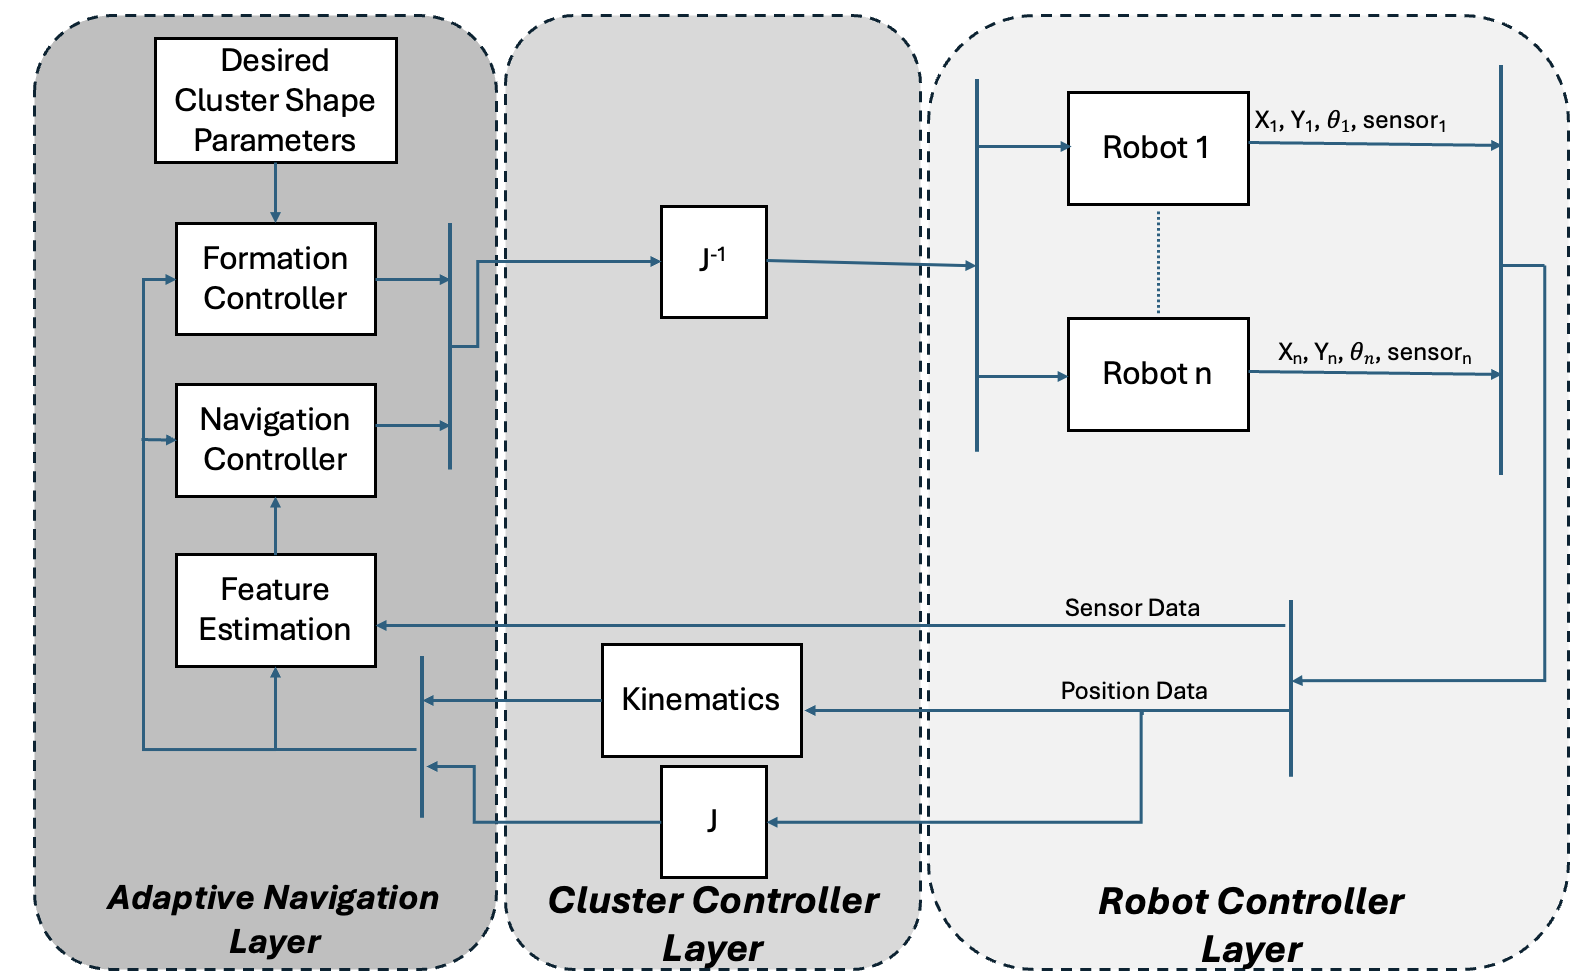
\includegraphics[width=\columnwidth]{figures/control_architecture.png}
    \caption{Three-layer control architecture\DIFdelbeginFL \DIFdelFL{. The }\DIFdelendFL \DIFaddbeginFL \DIFaddFL{: }\DIFaddendFL adaptive navigation \DIFdelbeginFL \DIFdelFL{layer }\DIFdelendFL (left)\DIFdelbeginFL \DIFdelFL{estimates the field and generates the cluster command}\DIFdelendFL ,
    \DIFdelbeginFL \DIFdelFL{the
    }\DIFdelendFL cluster controller \DIFdelbeginFL \DIFdelFL{layer }\DIFdelendFL (center)\DIFdelbeginFL \DIFdelFL{maps between cluster and robot space}\DIFdelendFL , and \DIFdelbeginFL \DIFdelFL{the }\DIFdelendFL robot controller \DIFdelbeginFL \DIFdelFL{layer }\DIFdelendFL (right)\DIFdelbeginFL \DIFdelFL{actuates each robot and reports
    its position and field sample}\DIFdelendFL . The contents
    of the feature estimation and navigation controller blocks are new in
    this paper.}
    \label{fig:control_architecture}
\end{figure}

\begin{figure}[!tb]
    \centering
    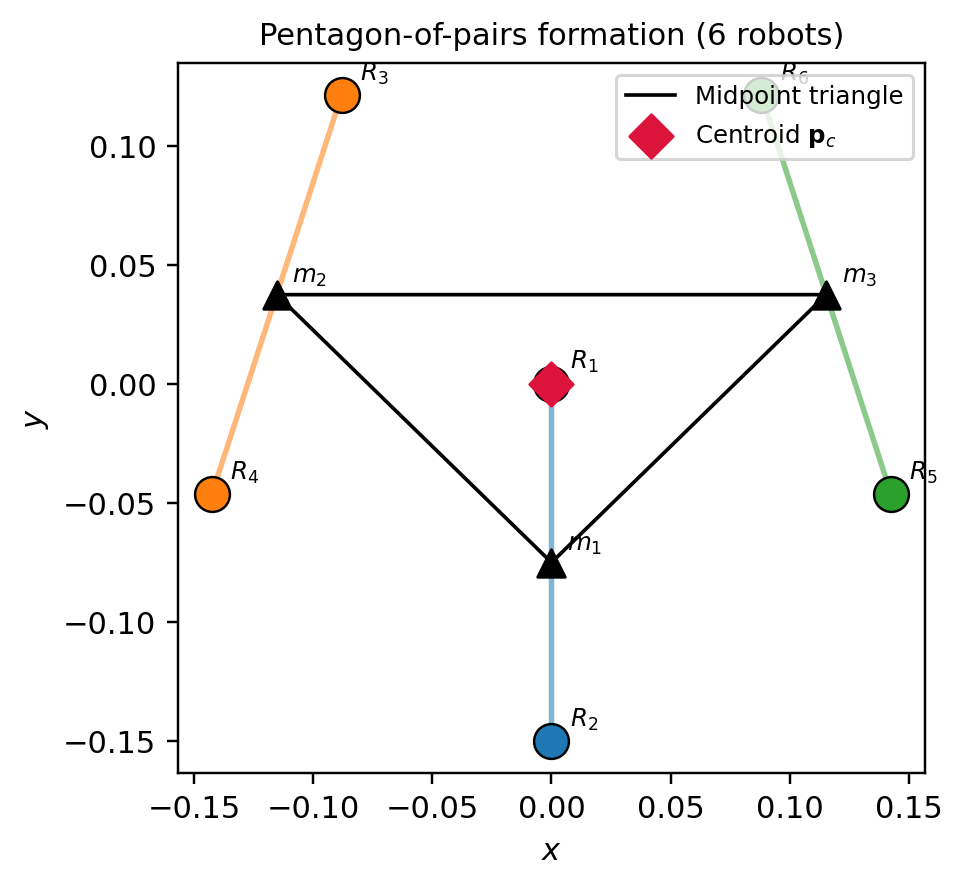
\includegraphics[width=0.8\columnwidth]{figures/pentagon_formation.png}
    \caption{Pentagon-plus-center formation. Robot 1 sits at the centroid
    $\mathbf{p}_c$ and robots 2 to 6 on a ring (dotted). The cluster
    variables shown are the pair separations $L_2$, $L_3$, $L_4$, a pair
    orientation $\theta_3$, the SAS parameters $(p, \beta, q)$ of the
    triangle of pair midpoints (squares), and the heading $\theta_c$.}
    \label{fig:pentagon}
\end{figure}

In the robot controller layer, each robot follows its velocity command
through \DIFdelbegin \DIFdel{a first-order lag, discretized at control period $\Delta t$ as the update
$\mathbf{v} \leftarrow \alpha_{\text{mom}}\mathbf{v} + (1 -
\alpha_{\text{mom}})\mathbf{v}^{\text{des}}$ with
$\alpha_{\text{mom}} = e^{-\Delta t/\tau}$. This momentum model was
identified in \mbox{%DIFAUXCMD
\cite{10} }\hskip0pt%DIFAUXCMD
}\DIFdelend \DIFaddbegin \DIFadd{the model that \mbox{%DIFAUXCMD
\cite{10} }\hskip0pt%DIFAUXCMD
identified }\DIFaddend on the Decabot indoor
omnidirectional testbed \cite{31,32}\DIFdelbegin \DIFdel{, and $\alpha_{\text{mom}} = 0.7$ at $\Delta t = 0.1$~sgives
$\tau \approx 0.28$~s, consistent with the identified lag . Each robot also
carries a speed limit and a stiction floor. }%DIFDELCMD < 

%DIFDELCMD < %%%
\DIFdelend \DIFaddbegin \DIFadd{. A robot reaches a share
$g = \rev{0.86}$ of its command after a delay $L = \rev{0.055}$~s, through
a first-order lag with time constant $\tau = \rev{0.02}$~s. It ignores
commands below a dead zone $v_c = 0.025$~m/s and is capped at 0.3~m/s. }\DIFaddend A
Python simulation integrates each robot's position by explicit Euler at the
control period \DIFdelbegin \DIFdel{. Table~\ref{tab:params} gives the two operating points,
fixed across all experiments unless noted}\DIFdelend \DIFaddbegin \DIFadd{$\Delta t = 0.1$~s. The simulation code and the scripts
behind every figure are available from the authors on request}\DIFaddend .

\DIFdelbegin %DIFDELCMD < \begin{table}[!t]
%DIFDELCMD < %%%
%DIFDELCMD < \caption{%
{%DIFAUXCMD
\DIFdelFL{Operating points. The double-gyre column is non-dimensional,
with one time unit equal to one second of the Decabot's identified
dynamics.}}
%DIFAUXCMD
%DIFDELCMD < \label{tab:params}
%DIFDELCMD < \centering
%DIFDELCMD < \begin{tabular}{llll}
%DIFDELCMD < \hline
%DIFDELCMD < Parameter & Double gyre & Ocean & Units \\
%DIFDELCMD < \hline
%DIFDELCMD < $c_{\max}$              & 0.04  & 0.033  & length/time \\
%DIFDELCMD < $k$                     & 3.0   & 1.94   & none \\
%DIFDELCMD < $\rho$                  & 0.075 & 0.098  & length (5.0 km) \\
%DIFDELCMD < $v_{\text{max,robot}}$  & 0.3   & 0.3    & length/time \\
%DIFDELCMD < $v_{\text{stiction}}$   & 0.025 & 0.002  & length/time \\
%DIFDELCMD < $\alpha_{\text{mom}}$   & 0.7   & 0      & none \\
%DIFDELCMD < $c_{\mathrm{crest}}$    & 0.1   & 0.1    & none \\
%DIFDELCMD < $g_\perp$              & 1.0   & 1.0    & length$^2$ \\
%DIFDELCMD < $q_{\mathrm{cap}}$      & 0.03  & 0.03   & none \\
%DIFDELCMD < \hline
%DIFDELCMD < \end{tabular}
%DIFDELCMD < \end{table}
%DIFDELCMD < 

%DIFDELCMD < %%%
\DIFdelend \subsection{The $D$ Tracker}
\label{sec:sep_controller}

The $D$ tracker is built for a mountain pass in $D$. Two minima are
joined by a trench that rises to a saddle point of $D$, the crest. On the
benchmark the trench is the separatrix and the minima are the flow saddles
(Fig.~\ref{fig:dg_fields}(b)). The tracker steers the centroid onto the
trench, \DIFdelbegin \DIFdel{along it }\DIFdelend over the crest, and down toward the next minimum\DIFdelbegin \DIFdel{. It
does so with two channels, one }\DIFdelend \DIFaddbegin \DIFadd{, with one channel
}\DIFaddend across the trench and one along it.

Across a trench $D$ curves upward, and along it $D$ can curve either way.
The tracker reads both directions from the eigenvectors of the fitted
Hessian, $\hat{\mathbf{H}}_{D,0}\mathbf{w}_j = \lambda_j \mathbf{w}_j$,
with $\|\mathbf{w}_j\| = 1$ and $\lambda_1 \leq \lambda_2$. The
eigenvector $\mathbf{w}_2$ points across the trench and $\mathbf{w}_1$
along it, signed by $\hat{\mathbf{v}}_0^\top \mathbf{w}_1 \geq 0$ to point
downstream, where $\hat{\mathbf{v}}_0 = (\hat{a}_1, \hat{b}_1)$ is the
measured flow at the centroid. This \DIFdelbegin \DIFdel{is }\DIFdelend \DIFaddbegin \DIFadd{follows }\DIFaddend the height-ridge definition
of a trench \cite{33}, \DIFdelbegin \DIFdel{a curve on which the gradient is orthogonal to the Hessian eigenvector of the larger eigenvalue, which is positive.
The identification is exact on the
benchmark, where $\mathbf{H}_D$ is diagonal, and approximate in general.
}\DIFdelend \DIFaddbegin \DIFadd{and on the benchmark the fitted eigenvectors lie
close to the true trench directions (Section~\ref{sec:dg_example}).
}\DIFaddend 

Away from the crest, both channels take Newton steps of the fitted
quadratic\DIFdelbegin \DIFdel{along their eigenvectors. The across-trench channel steps
toward the bottom of the trench, a distance
}\DIFdelend \DIFaddbegin \DIFadd{, }\DIFaddend $-\mathbf{w}_2^\top\hat{\mathbf{g}}_0/\lambda_2$ \DIFdelbegin \DIFdel{along $\mathbf{w}_2$. The
along-trench channel uses the
same ratio in magnitude,
}\DIFdelend \DIFaddbegin \DIFadd{toward the
trench bottom and }\DIFaddend $|\mathbf{w}_1^\top\hat{\mathbf{g}}_0|/|\lambda_1|$
along \DIFdelbegin \DIFdel{$\mathbf{w}_1$}\DIFdelend \DIFaddbegin \DIFadd{it}\DIFaddend , which slows the cluster as it nears the crest.

At the crest the along-trench gradient vanishes, and the measured flow
carries the cluster over instead. The \DIFdelbegin \DIFdel{crest is a saddle point of $D$, so
the tracker detects it }\DIFdelend \DIFaddbegin \DIFadd{tracker detects the crest }\DIFaddend as a
fitted saddle \DIFaddbegin \DIFadd{of $D$ }\DIFaddend whose stationary point lies inside the formation\DIFdelbegin \DIFdel{. The }\DIFdelend \DIFaddbegin \DIFadd{, a
}\DIFaddend crest set $\mathcal{B}$ \DIFdelbegin \DIFdel{is the set of points
where }\begin{displaymath}
    \DIFdel{\lambda_1\lambda_2 < 0
    \quad\text{and}\quad
    \bigl\|\hat{\mathbf{H}}_{D,0}^{-1}\,\hat{\mathbf{g}}_0\bigr\|
        < c_{\mathrm{crest}}\,\rho.
    %DIFDELCMD < \label{eq:band}%%%
}\end{displaymath}%DIFAUXCMD
\DIFdelend \DIFaddbegin \DIFadd{where $\lambda_1\lambda_2 < 0$ and
$\|\hat{\mathbf{H}}_{D,0}^{-1}\hat{\mathbf{g}}_0\| < c_{\mathrm{crest}}\,\rho$.
}\DIFaddend The left side \DIFdelbegin \DIFdel{of the second test }\DIFdelend is the Newton step to the stationary point, so
$c_{\mathrm{crest}}$ is a fraction of the formation radius and needs no
knowledge of the field's scale.
\DIFdelbegin \DIFdel{The second test is evaluated only
when $\lambda_1\lambda_2 < 0$, where $\hat{\mathbf{H}}_{D,0}$ is invertible,
and the step is solved exactly. Near the boundary between indefinite and
definite regions an eigenvalue approaches zero, the step grows without
bound, and the test fails, so no pseudo-inverse is needed.
}\DIFdelend 

Combining the two channels, the crest test selects the along-trench \DIFdelbegin \DIFdel{speed,
}\DIFdelend \DIFaddbegin \DIFadd{term,
}\DIFaddend \begin{equation}
    v_\parallel =
    \DIFdelbegin %DIFDELCMD < \begin{cases}
%DIFDELCMD <         \hat{\mathbf{v}}_0^\top \mathbf{w}_1,
%DIFDELCMD <             & \mathbf{p}_c \in \mathcal{B}, \\[6pt]
%DIFDELCMD <         \dfrac{|\mathbf{w}_1^\top \hat{\mathbf{g}}_0|}{|\lambda_1|},
%DIFDELCMD <             & \text{otherwise},
%DIFDELCMD <     \end{cases}%%%
\DIFdelend \DIFaddbegin \begin{cases}
        T\,\hat{\mathbf{v}}_0^\top \mathbf{w}_1,
            & \mathbf{p}_c \in \mathcal{B}, \\[6pt]
        \dfrac{|\mathbf{w}_1^\top \hat{\mathbf{g}}_0|}{|\lambda_1|},
            & \text{otherwise},
    \end{cases}\DIFaddend 
    \label{eq:vpar}
\end{equation}
and the centroid velocity command is
\begin{equation}
    \dot{\mathbf{p}}_c = k\Bigl[
    \underbrace{\mathrm{sat}(v_\parallel)\,\mathbf{w}_1}_{\text{along the trench}}
    + \underbrace{\mathrm{sat}\!\left(-\frac{\mathbf{w}_2^\top
      \hat{\mathbf{g}}_0}{\lambda_2}\right)\mathbf{w}_2}_{\text{across the trench}}\Bigr].
    \label{eq:d_law}
\end{equation}
\DIFdelbegin \DIFdel{Here $k$ is a navigation gain and
}\DIFdelend \DIFaddbegin \DIFadd{Every term in the brackets is a distance, with $T$ one time unit in the
crest branch, so the navigation gain $k$ has units of inverse time. The
function }\DIFaddend $\mathrm{sat}(c) = c_{\max}\tanh(c/c_{\max})$ saturates each
channel at \DIFdelbegin \DIFdel{speed }\DIFdelend \DIFaddbegin \DIFadd{the distance }\DIFaddend $c_{\max}$, which caps the centroid speed at
$\sqrt{2}\,k\,c_{\max}$. \DIFdelbegin \DIFdel{The same saturation }\DIFdelend \DIFaddbegin \DIFadd{It also }\DIFaddend bounds each Newton step where its
eigenvalue nears zero\DIFaddbegin \DIFadd{, and each eigenvalue in a denominator is floored at
$10^{-9}$ in magnitude, so no step divides by zero}\DIFaddend . Both branches of
$v_\parallel$ are nonnegative, so the along-trench motion never opposes
the flow\DIFdelbegin \DIFdel{. The same law runs }\DIFdelend \DIFaddbegin \DIFadd{, and }\DIFaddend where the fitted Hessian is definite \DIFdelbegin \DIFdel{and no trench exists, with $\mathbf{w}_1$ still the eigenvector of the smaller eigenvalue, so the tracker needs no separate
rule there}\DIFdelend \DIFaddbegin \DIFadd{the same law runs
unchanged}\DIFaddend .

The tracker stops at the end of the pass with the critical point test of
\cite{10}\DIFdelbegin \DIFdel{. On the benchmark the minima of $D$ are the flow saddles, and
the test }\DIFdelend \DIFaddbegin \DIFadd{, which }\DIFaddend fires when the fitted flow has a saddle inside the
formation,
\DIFdelbegin \begin{displaymath}
    \DIFdel{\det\hat{\mathbf{J}}_0 < 0
    \quad\text{and}\quad
    \bigl\|\hat{\mathbf{J}}_0^{-1}\hat{\mathbf{v}}_0\bigr\| < \rho,
    \label{eq:d_capture}
}\end{displaymath}%DIFAUXCMD
\DIFdelend \DIFaddbegin \DIFadd{$\det\hat{\mathbf{J}}_0 < 0$ and
$\|\hat{\mathbf{J}}_0^{-1}\hat{\mathbf{v}}_0\| < \rho$, }\DIFaddend where $\hat{\mathbf{J}}_0$ is the fitted Jacobian at the centroid and
$\hat{\mathbf{J}}_0^{-1}\hat{\mathbf{v}}_0$ is the Newton step to the
stagnation point. The test uses only the zeroth- and first-order
coefficients, the least noisy the fit returns\DIFaddbegin \DIFadd{, and certifies a saddle of
the fitted linear flow, which on the benchmark is the flow saddle at the
end of the trench}\DIFaddend . Once it passes, the tracker
holds for the rest of the run with the attraction law of \cite{10},
\DIFdelbegin \begin{displaymath}
    \DIFdel{\dot{\mathbf{p}}_c = k\,\mathrm{sat}\bigl(-\hat{\mathbf{J}}_0^{-1}\hat{\mathbf{v}}_0\bigr),
    \label{eq:d_hold}
}\end{displaymath}%DIFAUXCMD
\DIFdelend \DIFaddbegin \DIFadd{$\dot{\mathbf{p}}_c = k\,\mathrm{sat}(-\hat{\mathbf{J}}_0^{-1}\hat{\mathbf{v}}_0)$
}\DIFaddend with $\mathrm{sat}$ applied to each component\DIFdelbegin \DIFdel{, which steers the centroid to
the fitted stagnation point from the same coefficients as the test}\DIFdelend . Both read the measured
flow, so neither is objective.

\DIFdelbegin \DIFdel{The across-trench channel drives the cluster to the fitted trench bottom
with the command $\mathbf{w}_2^\top\dot{\mathbf{p}}_c = k\,\mathrm{sat}(e)$,
where $e = -\mathbf{w}_2^\top\hat{\mathbf{g}}_0/\lambda_2$ is the signed
distance to the trench bottom. Assuming a stationary estimate, the
Lyapunov function $V = \tfrac{1}{2}e^2$ yields $\dot{V} = -k\,e\,\mathrm{sat}(e) < 0$ for
$e \neq 0$ under realized kinematics, guaranteeing local convergence. This descent assumes positive
curvature ($\lambda_2 > 0$), which holds intrinsically unless inverted by
noise.
}%DIFDELCMD < 

%DIFDELCMD < %%%
\DIFdelend \subsection{The $s_1$ Tracker}
\label{sec:s1_controller}

The fitted $\hat{s}_1$ is concave for every field and formation
(Section~\ref{sec:surrogates})\DIFdelbegin \DIFdel{. It }\DIFdelend \DIFaddbegin \DIFadd{, so it }\DIFaddend never shows the upward curvature a
trench has across it, and the \DIFdelbegin \DIFdel{Newton step that returns the }\DIFdelend $D$ tracker\DIFdelbegin \DIFdel{to
its trench }\DIFdelend \DIFaddbegin \DIFadd{'s Newton step }\DIFaddend has no counterpart
here. The tracker instead builds both channels from $\nabla\hat{s}_1$ and
the strain eigenframe.

The trench tangent is a strain eigenvector (Section~\ref{sec:surrogates}),
and the tracker must choose between $\mathbf{e}_1$ and $\mathbf{e}_2$ at
every step. On the trench the transverse derivative of $s_1$ vanishes, so
$\nabla\hat{s}_1$ lies nearly along the trench away from a stationary
point. The tangent is the eigenvector most nearly parallel to it, signed
against a reference,
\begin{equation}
    \mathbf{t}_{\mathrm{raw}} =
    \arg\max_{\mathbf{e} \in \{\mathbf{e}_1, \mathbf{e}_2\}}
    \bigl\lvert \nabla\hat{s}_1^\top \mathbf{e} \bigr\rvert,
    \qquad
    \mathbf{t} = \mathrm{sgn}\bigl(\mathbf{t}_{\mathrm{ref}}^\top
    \mathbf{t}_{\mathrm{raw}}\bigr)\,\mathbf{t}_{\mathrm{raw}},
    \label{eq:tangent_select}
\end{equation}
where $\mathbf{t}_{\mathrm{ref}}$ is the previous step's tangent
(Fig.~\ref{fig:s1_channels}(a)). \DIFdelbegin \DIFdel{On a trench that is not an OECS, the
rule takes the nearer eigenvector. }\DIFdelend The first ride step has no previous
tangent, so the measured flow $\hat{\mathbf{v}}_0$ serves as
$\mathbf{t}_{\mathrm{ref}}$\DIFaddbegin \DIFadd{, the one non-objective input. After that an
observer rotating at rate $\Omega$ turns the stored tangent by only
$\Omega\,\Delta t$ between steps, far from the $90^\circ$ at which the
sign test would flip, so every later input is objective}\DIFaddend .
\DIFdelbegin \DIFdel{Because the measured flow is not objective, it seeds the ride direction only once.
}\DIFdelend 

From the first step, the command pairs a constant-speed ride along
$\mathbf{t}$ with gradient descent across the trench,
\begin{equation}
    \dot{\mathbf{p}}_c = k\Bigl[
    \underbrace{\mathrm{sat}(c_{\max})\,\mathbf{t}}_{\text{along the trench}}
    + \underbrace{\mathrm{sat}\bigl(-g_\perp\,\mathbf{t}_\perp^\top
      \nabla\hat{s}_1\bigr)\,\mathbf{t}_\perp}_{\text{across the trench}}\Bigr],
    \label{eq:s1_law}
\end{equation}
with transverse gain $g_\perp$ and $\mathbf{t}_\perp$ the unit normal to
$\mathbf{t}$. \DIFaddbegin \DIFadd{As in (\ref{eq:d_law}) each bracketed term is a distance, so
$g_\perp$ carries units of length squared times time. }\DIFaddend The cluster rides at
speed $k\,c_{\max}\tanh 1$ throughout\DIFdelbegin \DIFdel{.
The across-trench channel sees only the component of $\nabla\hat{s}_1$
along $\mathbf{t}_\perp$ }\DIFdelend \DIFaddbegin \DIFadd{, and descends only across the
trench }\DIFaddend (Fig.~\ref{fig:s1_channels}(b))\DIFdelbegin \DIFdel{, so the cluster
descends only across the trench}\DIFdelend .

The ride speed does not depend on the slope, so \DIFdelbegin \DIFdel{on the benchmark the
}\DIFdelend \DIFaddbegin \DIFadd{the }\DIFaddend cluster crosses the
crest without the crest test the $D$ tracker needs. In incompressible flow
$s_1 = -r \leq 0$ \DIFdelbegin \DIFdel{, which }\DIFdelend reaches zero only at an isotropic point, where the
strain vanishes. \DIFdelbegin \DIFdel{Such }\DIFdelend \DIFaddbegin \DIFadd{In general such }\DIFaddend a point is \DIFdelbegin \DIFdel{in general an isolatedpeak, so the }\DIFdelend \DIFaddbegin \DIFadd{isolated, so a }\DIFaddend crest is a
smooth saddle \DIFdelbegin \DIFdel{with $r > 0$. There }\DIFdelend \DIFaddbegin \DIFadd{where }\DIFaddend $\nabla\hat{s}_1$ vanishes \DIFdelbegin \DIFdel{, }\DIFdelend and the tangent rule is
least reliable\DIFdelbegin \DIFdel{, as it is near a
minimum. In special flows, such as one whose }\DIFdelend \DIFaddbegin \DIFadd{. On the benchmark the }\DIFaddend shear strain vanishes identically, the
isotropic points form curves, and the crest \DIFdelbegin \DIFdel{can sit }\DIFdelend \DIFaddbegin \DIFadd{sits }\DIFaddend on one at a kink of
$s_1$. \DIFdelbegin %DIFDELCMD < 

%DIFDELCMD < %%%
\DIFdel{The tangent changes eigenvectoronly at an isotropic point}\DIFdelend \DIFaddbegin \DIFadd{There the tangent swaps eigenvector}\DIFaddend , and the rule follows the swap
with no dedicated test, since $\nabla\hat{s}_1$ stays large on either
side\DIFdelbegin \DIFdel{of the kink. On the benchmark,
$\mathbf{S} = \mathrm{diag}(u_x, -u_x)$ has its eigenvectors on the
coordinate axes wherever $u_x \neq 0$. On the upper segment of the
separatrix }\DIFdelend \DIFaddbegin \DIFadd{. Above the origin }\DIFaddend $u_x < 0$, so the trench follows $\mathbf{e}_2$ and
is an attracting OECS\DIFdelbegin \DIFdel{. On the lower segment }\DIFdelend \DIFaddbegin \DIFadd{; below it }\DIFaddend $u_x > 0$, so it follows $\mathbf{e}_1$
and is a repelling OECS.
\DIFdelbegin \DIFdel{The two meet at the origin, an
isotropic point of $\mathbf{S}$ where the crest sits at a kink.
}\DIFdelend 

The tracker stops at a minimum by a gradient test. The concave fit cannot
certify a minimum, but the fitted gradient tracks the true gradient even
where the fitted curvature has the wrong sign. Each end of the trench is
a true two-dimensional minimum of $s_1$, so a gradient that is small
against the depth suffices. Capture requires $\hat{s}_1 < 0$ and
\DIFdelbegin \begin{displaymath}
    \DIFdel{q = \frac{\rho\,\|\nabla\hat{s}_1\|}{|\hat{s}_1|} < q_{\mathrm{cap}},
    \label{eq:s1_capture}
}\end{displaymath}%DIFAUXCMD
\DIFdelend \DIFaddbegin \DIFadd{$q = \rho\,\|\nabla\hat{s}_1\|/|\hat{s}_1| < q_{\mathrm{cap}}$, }\DIFaddend where $q$ is the fraction by which $\hat{s}_1$ changes across the
footprint. The ratio is dimensionless, so $q_{\mathrm{cap}}$ needs no
knowledge of the field's strain rate. It is large along the ride and wherever $\hat{s}_1$ nears zero, as at an isotropic point or a
gyre center\DIFdelbegin \DIFdel{. It is also }\DIFdelend \DIFaddbegin \DIFadd{, but }\DIFaddend small at any \DIFdelbegin \DIFdel{other stationary point of $\hat{s}_1$
}\DIFdelend \DIFaddbegin \DIFadd{stationary point }\DIFaddend with $\hat{s}_1 < 0$, so
the test can \DIFaddbegin \DIFadd{also }\DIFaddend pass at a smooth crest. On the benchmark the crest sits
on an isotropic point, \DIFdelbegin \DIFdel{where $\hat{s}_1 = 0$, }\DIFdelend so only the minima pass. Once the test passes, the
tracker
drops the ride term and descends $\hat{s}_1$ for the rest of the run with
$\dot{\mathbf{p}}_c = -k\,\mathrm{sat}_{\mathrm{v}}(g_\perp\nabla\hat{s}_1)$,
where $\mathrm{sat}_{\mathrm{v}}(\mathbf{a}) =
\mathrm{sat}(\|\mathbf{a}\|)\,\mathbf{a}/\|\mathbf{a}\|$ saturates the
vector's magnitude and preserves its direction, which keeps the descent
independent of the coordinate axes.
\DIFdelbegin \DIFdel{If noise trips the test early on the trench, the descent
still carries the cluster down the trench to the minimum.
}\DIFdelend 

\begin{figure}[!tb]
    \centering
    \DIFdelbeginFL %DIFDELCMD < \includegraphics[width=\columnwidth]{figures/s1_channels.png}
%DIFDELCMD <     %%%
\DIFdelendFL \DIFaddbeginFL \includegraphics[width=\columnwidth]{figures/s1_channels_d14.png}
    \DIFaddendFL \caption{The two channels of the $s_1$ tracker \DIFdelbeginFL \DIFdelFL{, }\DIFdelendFL on the benchmark trench
    \DIFdelbeginFL \DIFdelFL{at }\DIFdelendFL $x = 0$. (a) Tangent selection\DIFdelbeginFL \DIFdelFL{. At each sample }\DIFdelendFL \DIFaddbeginFL \DIFaddFL{: }\DIFaddendFL the strain eigenframe\DIFdelbeginFL \DIFdelFL{is
    drawn}\DIFdelendFL , \DIFdelbeginFL \DIFdelFL{the }\DIFdelendFL selected
    eigenvector heavy\DIFdelbeginFL \DIFdelFL{and the rejected one light}\DIFdelendFL , with $\nabla\hat{s}_1$ in orange. The \DIFdelbeginFL \DIFdelFL{argmax takes
    }\DIFdelendFL \DIFaddbeginFL \DIFaddFL{tangent is
    }\DIFaddendFL $\mathbf{e}_2$ on the attracting segment and $\mathbf{e}_1$ on the
    repelling \DIFdelbeginFL \DIFdelFL{segment}\DIFdelendFL \DIFaddbeginFL \DIFaddFL{one}\DIFaddendFL , swapping \DIFdelbeginFL \DIFdelFL{through the isotropic point }\DIFdelendFL at the origin. (b) The command\DIFdelbeginFL \DIFdelFL{. Travel }\DIFdelendFL \DIFaddbeginFL \DIFaddFL{: an open-loop
    ride }\DIFaddendFL along $\mathbf{t}$ \DIFdelbeginFL \DIFdelFL{is open loop at cruise
    speed, while }\DIFdelendFL \DIFaddbeginFL \DIFaddFL{and a }\DIFaddendFL descent \DIFdelbeginFL \DIFdelFL{uses only the component of $\nabla\hat{s}_1$
    along $\mathbf{t}_\perp$, so the cluster descends only }\DIFdelendFL across \DIFdelbeginFL \DIFdelFL{the
    trench}\DIFdelendFL \DIFaddbeginFL \DIFaddFL{it}\DIFaddendFL .}
    \label{fig:s1_channels}
\end{figure}

\DIFdelbegin \DIFdel{The across-trench channel drives the cluster to the trench using the command $\mathbf{t}_\perp^\top\dot{\mathbf{p}}_c =
-k\,\mathrm{sat}(g_\perp\mathbf{t}_\perp^\top\nabla\hat{s}_1)$. For signed
transverse distance $n$, assuming realized kinematics and an accurate
gradient fit, the Lyapunov function $V = \tfrac{1}{2}n^2$ yields
$\dot{V} = -k\,n\,\mathrm{sat}(g_\perp\mathbf{t}_\perp^\top\nabla\hat{s}_1) < 0$
for $n \neq 0$, guaranteeing local convergence. It also bounds the cluster near the trench under a disturbance smaller than }\DIFdelend \DIFaddbegin \subsection{\DIFadd{Closed-Loop Behavior}}
\label{sec:closed_loop}

\DIFadd{Both trackers pull the cluster onto the trench through one saturated loop
across it, of the form \mbox{%DIFAUXCMD
\cite{10} }\hskip0pt%DIFAUXCMD
analyzed on the same robots. With the
delay and gain of Section~\ref{sec:arch}, the sampled loop is
exponentially stable for loop gains below $1/(gL) = \rev{21.1}$ per unit
time, or \rev{16.1} with the lag included, and as a stable linear loop it
keeps }\DIFaddend the across-trench \DIFdelbegin \DIFdel{command at some distance from it, a bound always below $k\,c_{\max}$. Because no fitted
curvatureenters, this descent relies only on the true upward curvature
of }\DIFdelend \DIFaddbegin \DIFadd{error bounded under a bounded estimate error
\mbox{%DIFAUXCMD
\cite{10}}\hskip0pt%DIFAUXCMD
. The result is local.
}

\DIFadd{Neither channel is exactly linear. The $D$ tracker divides by the fitted
curvature, so its gain is $k$ times the ratio of true to fitted curvature
across }\DIFaddend the trench, \DIFdelbegin \DIFdel{which holds intrinsically, even at smooth crests, unless an
intersecting curve of isotropic points flattens the
trench, leaving the tangent rideto carry the cluster across alone.
}\DIFdelend \DIFaddbegin \DIFadd{$1/\sin^2\pi y_f$ on the benchmark. The gain is
$k = 3$ at the crest and exceeds the bound only within \rev{0.14} of the
saddles (Section~\ref{sec:dg_example}). The $s_1$ tracker's gain is
$k\,g_\perp\,\partial^2 s_1/\partial n^2$, or $3\pi^4 A\,|\cos\pi y_f|$
on the benchmark, which exceeds the bound for $|y| > \rev{0.19}$ and
reaches \rev{29} at the saddles. Each channel saturates a few thousandths
from the trench, which keeps any resulting oscillation in a narrow band.
At the end of the ride, the $D$ tracker's hold is the
attraction law of \mbox{%DIFAUXCMD
\cite{10}}\hskip0pt%DIFAUXCMD
, so the cluster settles inside the friction
ring $v_c/k = \rev{0.008}$ around the fitted stagnation point.
Table~\ref{tab:params} collects the operating points.
}\DIFaddend 

\DIFaddbegin \begin{table}[!t]
\caption{\DIFaddFL{Operating points. The double-gyre column is non-dimensional,
with one time unit equal to one second of the Decabot's identified
dynamics. The ocean column uses the scaling of the Santa Barbara Channel
trial.}}
\label{tab:params}
\centering
\begin{tabular}{llll}
\hline
Parameter & Double gyre & Ocean & Units \\
\hline
$k$                     & 3.0   & 1.94   & 1/time \\
$c_{\max}$              & 0.04  & 0.033  & length \\
$\rho$                  & 0.075 & 0.098  & length \\
$c_{\mathrm{crest}}$    & 0.1   & 0.1    & none \\
$g_\perp$               & 1.0   & 1.0    & length$^2\cdot$time \\
$q_{\mathrm{cap}}$      & 0.03  & 0.03   & none \\
robot $g$, $L$, $\tau$   & \rev{0.86}, \rev{0.055}, \rev{0.02} & 1, 0, 0 & --, time, time \\
dead zone $v_c$, cap     & 0.025, 0.3 & 0.002, 0.3 & length/time \\
\hline
\end{tabular}
\end{table}


\DIFaddend \section{Double-Gyre Benchmark}
\label{sec:dg_bench}

\subsection{Setup}

The double-gyre experiments use the steady field of
Section~\ref{sec:dg_example} and the nominal formation, with ring radius
$\rho = 0.075$. Trials vary only the initial heading, set to zero in the
noise-free runs and drawn uniformly from $[0, 2\pi)$ in the Monte Carlo
sweeps\DIFdelbegin \DIFdel{. All trials run }\DIFdelend \DIFaddbegin \DIFadd{, }\DIFaddend for up to 500 steps. \DIFdelbegin %DIFDELCMD < 

%DIFDELCMD < %%%
\DIFdelend The task is to ride the separatrix downstream
and capture the saddle at its end, $\mathbf{p}^*_1 = (0, -0.5)$\DIFdelbegin \DIFdel{. A }\DIFdelend \DIFaddbegin \DIFadd{; a }\DIFaddend run
that ends at $\mathbf{p}^*_2$ has ridden against the flow and fails. \DIFdelbegin \DIFdel{Performance is scored on
acquisition, saddle capture, and straddle retention. }\DIFdelend A
run acquires the separatrix at the first of ten consecutive
steps with its centroid within 0.05 of $x = 0$. Noise-free trials stop once
the centroid has stayed within 0.06 of a flow saddle for 20 consecutive
steps, while noisy trials succeed if the centroid comes within 0.06 of
$\mathbf{p}^*_1$. \DIFdelbegin \DIFdel{In a separate check of 1260 longer
trials at three noise levels, every trial but one that reached a saddle
also held it for 20 consecutive steps. }\DIFdelend The formation straddles the separatrix when robots lie
on both sides of $x = 0$. Because losing the straddle is the failure
\cite{26} reports, we measure noise tolerance by retention, the fraction
of trials that succeed and never stop straddling the separatrix after
their first straddle.

\subsection{Clean Runs}
\label{sec:disc_clean}

\begin{figure}[!tb]
    \centering
    \DIFdelbeginFL %DIFDELCMD < \includegraphics[width=\columnwidth]{figures/traverse_vs_logic_c_seven.png}
%DIFDELCMD <     %%%
\DIFdelendFL \DIFaddbeginFL \includegraphics[width=\columnwidth]{figures/traverse_vs_logic_c_seven_d14.png}
    \DIFaddendFL \caption{$s_1$ tracker versus $D$ tracker from seven matched starts
    ($\bullet$), noise-free, at S1 $(-0.10, 0.30)$, S2 $(0.15, 0.25)$, S3 $(0, 0.35)$,
    S4 $(0, 0)$, S5 $(0, -0.25)$, S6 $(0.15, -0.15)$, and S7 $(0.10, -0.20)$\DIFdelbeginFL \DIFdelFL{. From above }\DIFdelendFL \DIFaddbeginFL \DIFaddFL{,
    each ending at }\DIFaddendFL the \DIFdelbeginFL \DIFdelFL{origin both
    traverse the separatrix through the isotropic point there. Both
    trackers capture and hold the }\DIFdelendFL downstream saddle ($\times$\DIFdelbeginFL \DIFdelFL{)}\DIFdelendFL , \DIFdelbeginFL \DIFdelFL{ending at the
    }\DIFdelendFL squares\DIFaddbeginFL \DIFaddFL{)}\DIFaddendFL . \DIFaddbeginFL \DIFaddFL{Shading marks
    the 0.1 cells from which a start reaches that saddle in at least 90\%
    (darker) or 50\% (lighter) of random headings, over \rev{8000}
    noise-free starts per tracker.}\DIFaddendFL }
    \label{fig:traverse_vs_logic_c}
\end{figure}

\begin{figure}[!tb]
    \centering
    \DIFdelbeginFL %DIFDELCMD < \includegraphics[width=\columnwidth]{figures/separatrix_formation_seven.png}
%DIFDELCMD <     %%%
\DIFdelendFL \DIFaddbeginFL \includegraphics[width=\columnwidth]{figures/separatrix_formation_seven_d14.png}
    \DIFaddendFL \caption{The six robots from start S1 (star) under both trackers,
    zoomed to the separatrix $x = 0$ (dashed)\DIFdelbeginFL \DIFdelFL{. Thin lines are }\DIFdelendFL \DIFaddbeginFL \DIFaddFL{: }\DIFaddendFL robot paths \DIFdelbeginFL \DIFdelFL{and }\DIFdelendFL \DIFaddbeginFL \DIFaddFL{(thin), }\DIFaddendFL the
    \DIFdelbeginFL \DIFdelFL{heavy line is the }\DIFdelendFL centroid \DIFdelbeginFL \DIFdelFL{. Outlines mark the
    pentagon-plus-center formation at the start}\DIFdelendFL \DIFaddbeginFL \DIFaddFL{(heavy)}\DIFaddendFL , \DIFdelbeginFL \DIFdelFL{during the ride, }\DIFdelendFL and \DIFdelbeginFL \DIFdelFL{at
    }\DIFdelendFL the \DIFdelbeginFL \DIFdelFL{downstream saddle ($\times$)}\DIFdelendFL \DIFaddbeginFL \DIFaddFL{formation at four instants}\DIFaddendFL .}
    \label{fig:formation}
\end{figure}

Without noise, both trackers acquire the separatrix, traverse it in the
same direction, and capture the downstream saddle from all seven matched
starts (Fig.~\ref{fig:traverse_vs_logic_c}). Three starts lie on the
separatrix, at heights $0.35$, $0$, and $-0.25$\DIFdelbegin \DIFdel{. Four }\DIFdelend \DIFaddbegin \DIFadd{, and four }\DIFaddend lie off it by
$1.3\rho$ or $2\rho$, \DIFdelbegin \DIFdel{two above the origin and two below, and none of these straddles
the separatrix }\DIFdelend \DIFaddbegin \DIFadd{none straddling it }\DIFaddend at the first step. Both \DIFdelbegin \DIFdel{trackers }\DIFdelend acquire
the separatrix \DIFdelbegin \DIFdel{from all seven starts }\DIFdelend in 0 to 10 steps. Runs from above the origin \DIFdelbegin \DIFdel{then
}\DIFdelend ride the upper
segment\DIFdelbegin \DIFdel{to }\DIFdelend \DIFaddbegin \DIFadd{, an attracting OECS, through }\DIFaddend the isotropic point at the origin and
\DIFdelbegin \DIFdel{continue
}\DIFdelend onto the lower\DIFdelbegin \DIFdel{segment, }\DIFdelend \DIFaddbegin \DIFadd{, repelling one, }\DIFaddend with the formation straddling the
separatrix throughout (Fig.~\ref{fig:formation}). \DIFdelbegin \DIFdel{A run acquiring above the origin
therefore rides an attracting OECS to the origin and continues onto a
repelling one on the same primitive and scalar trench, and the }\DIFdelend \DIFaddbegin \DIFadd{The }\DIFaddend $s_1$ tracker
crosses the origin on ordinary tangent selection.

\DIFdelbegin \DIFdel{Both hold the downstream saddle $\mathbf{p}^*_1 = (0, -0.5)$ in all seven runs
}\DIFdelend \DIFaddbegin \DIFadd{The seven starts sample a wider basin }\DIFaddend (Fig.~\ref{fig:traverse_vs_logic_c}\DIFdelbegin \DIFdel{). The $s_1$ tracker
settles within
0.014 of
it and }\DIFdelend \DIFaddbegin \DIFadd{,
shading). Near mid-height both trackers reach $\mathbf{p}^*_1$ in at least
90\% of headings from any start within \rev{0.40} of the separatrix, more
than five formation radii, and the basin narrows to \rev{0.25} at
$|y| = 0.2$. Farther out the nearest trench need not be the separatrix,
and runs end elsewhere.
}

\DIFadd{Both hold $\mathbf{p}^*_1 = (0, -0.5)$ in all seven runs. The $D$ tracker
settles \rev{0.005} to \rev{0.006} from it, inside the friction ring of
Section~\ref{sec:closed_loop}, and the $s_1$ tracker within \rev{0.009}.
Where its gain exceeds the bound, the $s_1$ path wiggles about the
separatrix (Fig.~\ref{fig:formation}), a median \rev{0.004} from it below
$y = -0.19$ from S6 and S7, against under \rev{0.001} for }\DIFaddend the $D$
tracker\DIFdelbegin \DIFdel{within 0.004 to 0.006}\DIFdelend .

\subsection{Behavior Under Noise}
\label{sec:disc_noise}

\begin{figure}[!tb]
    \centering
    \DIFdelbeginFL %DIFDELCMD < \includegraphics[width=\columnwidth]{figures/noise_seven_starts_col.png}
%DIFDELCMD <     %%%
\DIFdelendFL \DIFaddbeginFL \includegraphics[width=\columnwidth]{figures/noise_seven_starts_col_d14.png}
    \DIFaddendFL \caption{Downstream-saddle success of both trackers from the seven starts of
    Fig.~\ref{fig:traverse_vs_logic_c}, one per row, \DIFdelbeginFL \DIFdelFL{$10^4$ }\DIFdelendFL \DIFaddbeginFL \DIFaddFL{\rev{1000} }\DIFaddendFL trials per point,
    with each tracker's retention \DIFdelbeginFL \DIFdelFL{, the fraction of trials that succeed and
    keep the straddle, }\DIFdelendFL dashed. \DIFdelbeginFL \DIFdelFL{S1 }\DIFdelendFL \DIFaddbeginFL \DIFaddFL{Ticks }\DIFaddendFL and \DIFdelbeginFL \DIFdelFL{S2 start off }\DIFdelendFL \DIFaddbeginFL \DIFaddFL{labels mark }\DIFaddendFL the \DIFdelbeginFL \DIFdelFL{separatrix above the origin}\DIFdelendFL \DIFaddbeginFL \DIFaddFL{noise
    level at which retention falls to 50\%}\DIFaddendFL , \DIFdelbeginFL \DIFdelFL{S3, S4, }\DIFdelendFL and \DIFdelbeginFL \DIFdelFL{S5
    on it, and S6 and S7 off it below the origin. Each }\DIFdelendFL \DIFaddbeginFL \DIFaddFL{each }\DIFaddendFL inset marks the start
    (dot)\DIFdelbeginFL \DIFdelFL{in the basin}\DIFdelendFL , \DIFdelbeginFL \DIFdelFL{with }\DIFdelendFL the separatrix\DIFdelbeginFL \DIFdelFL{dashed }\DIFdelendFL \DIFaddbeginFL \DIFaddFL{, }\DIFaddendFL and \DIFdelbeginFL \DIFdelFL{the downstream saddle
    }\DIFdelendFL $\mathbf{p}^*_1$ \DIFdelbeginFL \DIFdelFL{starred}\DIFdelendFL \DIFaddbeginFL \DIFaddFL{(star)}\DIFaddendFL . (a) Against
    $\sigma_{uv}$, $\sigma_p = 0$. (b) Against $\sigma_p$, $\sigma_{uv} = 0$.}
    \label{fig:flip_resolution}
\end{figure}

Both primitives sweep measurement and position noise separately from the
seven starts\DIFdelbegin \DIFdel{of Fig.~\ref{fig:traverse_vs_logic_c}, at $10^4$ }\DIFdelend \DIFaddbegin \DIFadd{, at \rev{1000} }\DIFaddend trials per noise level
\DIFdelbegin \DIFdel{from independent headings }\DIFdelend (Fig.~\ref{fig:flip_resolution})\DIFdelbegin \DIFdel{.
Without noise, both trackers
reach $\mathbf{p}^*_1$ in all $10^4$ trials from every start.
}%DIFDELCMD < 

%DIFDELCMD < %%%
\DIFdel{Both trackers }\DIFdelend \DIFaddbegin \DIFadd{, and both }\DIFaddend degrade smoothly as noise
grows\DIFdelbegin \DIFdel{, with no threshold at which
either suddenly fails.
From S3, the $D$ tracker's retention
falls from 99.4\% at $\sigma_{uv} = 0.0015$ to 23\% at $\sigma_{uv} = 0.03$,
while the $s_1$ tracker's falls from 85\% at $\sigma_{uv} = 0.00075$ to
under 1\% at $\sigma_{uv} = 0.004$}\DIFdelend .

\DIFdelbegin \DIFdel{Both trackers failat high noise for the same reason. Each }\DIFdelend \DIFaddbegin \DIFadd{The closed form of Section~\ref{sec:sensitivity} predicts where both must
fail. Each tracker }\DIFaddend steers on the second-order coefficients\DIFdelbegin \DIFdel{of the fit, which carry the most noise because
the fit recovers them from velocity differences divided by $\rho^2$. For
this formation }\DIFdelend \DIFaddbegin \DIFadd{, and }\DIFaddend each pure
second derivative carries a standard deviation of
$2.53\,\sigma_{uv}/\rho^2$\DIFdelbegin \DIFdel{. At }\DIFdelend \DIFaddbegin \DIFadd{, which at }\DIFaddend $\rho = 0.075$ \DIFdelbegin \DIFdel{this noise }\DIFdelend matches the largest
second derivative in the field, $\pi^3 A \approx 3.1$, near
$\sigma_{uv} = 0.007$. \DIFdelbegin \DIFdel{Beyond this level the fit cannot resolve even
the strongest curvature in the field, and by }\DIFdelend \DIFaddbegin \DIFadd{By }\DIFaddend $\sigma_{uv} = 0.01$ neither tracker \DIFdelbegin \DIFdel{retains more than 65\% of its }\DIFdelend \DIFaddbegin \DIFadd{keeps the
straddle in more than \rev{60}\% of }\DIFaddend trials from any start. \DIFaddbegin \DIFadd{The same form
predicts how formation size moves the limit. From S3 and S4, the $D$
tracker's 50\% retention level rises by a factor of \rev{5.0} and
\rev{4.7} from $\rho = 0.05$ to $0.075$ and is never reached at
$\rho = 0.1125$, and the $s_1$ tracker's rises by \rev{2.6} from
$\rho = 0.075$ to $0.1125$. Both beat the factor of 2.25 the coefficient
noise alone predicts, since a wider ring also straddles a larger offset,
so over this range the truncation error has not yet set the limit.
}\DIFaddend 

The $D$ tracker tolerates more noise \DIFdelbegin \DIFdel{than the $s_1$ tracker }\DIFdelend from every start, under both noise
types. Against measurement noise \DIFdelbegin \DIFdel{, the level at
which its retention falls to }\DIFdelend \DIFaddbegin \DIFadd{its }\DIFaddend 50\%
\DIFdelbegin \DIFdel{is 5.4 to 5.8 }\DIFdelend \DIFaddbegin \DIFadd{retention level is \rev{4.4} to \rev{5.6} }\DIFaddend times the $s_1$ tracker's above
the origin, \DIFdelbegin \DIFdel{4.2 }\DIFdelend \DIFaddbegin \DIFadd{\rev{3.5} }\DIFaddend times at it, and \DIFdelbegin \DIFdel{1.1 to 1.2 }\DIFdelend \DIFaddbegin \DIFadd{\rev{1.3} to \rev{1.5} }\DIFaddend times from S6
and S7\DIFdelbegin \DIFdel{.
From }\DIFdelend \DIFaddbegin \DIFadd{, and from }\DIFaddend S5 its retention never falls to 50\%. \DIFdelbegin \DIFdel{The
order reverses only at high noise }\DIFdelend \DIFaddbegin \DIFadd{Against position
noise the ratios are \rev{2.8} to \rev{4.9} and \rev{1.3} to \rev{1.4}.
Only }\DIFaddend from S6 and S7 \DIFdelbegin \DIFdel{, where the two }\DIFdelend \DIFaddbegin \DIFadd{do the }\DIFaddend retention curves cross\DIFdelbegin \DIFdel{near $\sigma_{uv} = 0.006$. }%DIFDELCMD < 

%DIFDELCMD < %%%
\DIFdel{The }\DIFdelend \DIFaddbegin \DIFadd{, near
$\sigma_{uv} = \rev{0.005}$. Halving $g_\perp$, which brings the }\DIFaddend $s_1$
tracker\DIFdelbegin \DIFdel{fails in two ways.
The main one }\DIFdelend \DIFaddbegin \DIFadd{'s gain under the bound of Section~\ref{sec:closed_loop}
everywhere, changes its retention by at most \rev{2.3} points.
}

\DIFadd{The $s_1$ tracker's main failure }\DIFaddend is a reversal\DIFdelbegin \DIFdel{, in which
the cluster turns around on the separatrix and rides it the wrong way. At
}\DIFdelend \DIFaddbegin \DIFadd{: at
}\DIFaddend $\sigma_{uv} = 0.002$, \DIFdelbegin \DIFdel{97 to 98\% of the $s_1$ }\DIFdelend \DIFaddbegin \DIFadd{\rev{96} to \rev{100}\% of its }\DIFaddend trials that miss
$\mathbf{p}^*_1$ end at $\mathbf{p}^*_2$\DIFdelbegin \DIFdel{, from every start. Even runs from below the origin therefore climb past it against the flow.
Reversals come from how the tracker keeps its direction. }\DIFdelend \DIFaddbegin \DIFadd{. }\DIFaddend The $D$ tracker re-signs its
direction every cycle against the measured flow\DIFdelbegin \DIFdel{. That flow is
not objective, so }\DIFdelend \DIFaddbegin \DIFadd{, while }\DIFaddend the $s_1$ tracker\DIFdelbegin \DIFdel{instead }\DIFdelend \DIFaddbegin \DIFadd{,
to stay objective, }\DIFaddend carries its sign forward\DIFdelbegin \DIFdel{from
step to step}\DIFdelend . Near the saddles \DIFdelbegin \DIFdel{, }\DIFdelend the
along-trench slope $\pi^3 A|\sin\pi y_f|$ that tangent selection relies on
goes to zero\DIFdelbegin \DIFdel{. One
noisy step there }\DIFdelend \DIFaddbegin \DIFadd{, so one noisy step }\DIFaddend can select the transverse eigenvector \DIFdelbegin \DIFdel{, after which the next step's sign is }\DIFdelend \DIFaddbegin \DIFadd{and
leave the next sign }\DIFaddend arbitrary. The \DIFdelbegin \DIFdel{$s_1$ capture holds whichever saddle
the ride reaches, including $\mathbf{p}^*_2$ after a reversal. The second
failure is subtler, reaching
$\mathbf{p}^*_1$ but losing the straddle on the way. From S5 at
$\sigma_{uv} = 0.01$, 77\% of the $s_1$ tracker's trials reach
$\mathbf{p}^*_1$ but only 33\% keep the straddle.
For the $D$ tracker the
two rates differ by at most 6 percentage points up to
$\sigma_{uv} = 0.005$.
}\DIFdelend \DIFaddbegin \DIFadd{chance of a first reversal per riding
step is \rev{0.13} in the top tenth of the separatrix and \rev{0.002} to
\rev{0.004} near the middle.
}\DIFaddend 

The $D$ tracker's \DIFdelbegin \DIFdel{lower tolerance }\DIFdelend \DIFaddbegin \DIFadd{smaller margin }\DIFaddend from S6 and S7 comes from \DIFdelbegin \DIFdel{the fitted
Hessianbecoming }\DIFdelend \DIFaddbegin \DIFadd{its fitted
Hessian, whose across-trench curvature falls short near the saddles
(Section~\ref{sec:dg_example}), so noise can make it }\DIFaddend definite before the
cluster reaches the separatrix. \DIFdelbegin \DIFdel{Because the fitted eigenvalues shrink toward the saddles, noise can make
$\hat{\mathbf{H}}_{D,0}$ definite during acquisition. }\DIFdelend At $\sigma_{uv} = 0.005$ this \DIFdelbegin \DIFdel{occurs in 92\% and
83}\DIFdelend \DIFaddbegin \DIFadd{happens in \rev{95}\% and
\rev{86}}\DIFaddend \% of trials from S6 and S7, \DIFdelbegin \DIFdel{and only 45\% and 51}\DIFdelend \DIFaddbegin \DIFadd{which meet the separatrix near
$y = -0.30$, and only \rev{32}\% and \rev{38}}\DIFaddend \% of those trials \DIFdelbegin \DIFdel{go on to }\DIFdelend reach
$\mathbf{p}^*_1$, against \DIFdelbegin \DIFdel{85\% for }\DIFdelend \DIFaddbegin \DIFadd{\rev{85}\% and \rev{81}\% of }\DIFaddend the rest. From S1
and S2\DIFdelbegin \DIFdel{the fitted
Hessian becomes definite in 75\%
and 83}\DIFdelend \DIFaddbegin \DIFadd{, which meet it inside $|y| < 0.25$, the same happens in \rev{75}\%
and \rev{84}}\DIFaddend \% of trials without changing success.
\DIFdelbegin \DIFdel{Runs from S1 and S2 meet the separatrix inside $|y| < 0.25$,
where the true $\mathbf{H}_D$ is indefinite, while runs from S6 and S7
meet it near $y = -0.30$, where it is definite.
}\DIFdelend 

\subsection{Behavior Under a Rotating Observer}
\label{sec:rotating}

\begin{figure}[!tb]
    \centering
    \DIFdelbeginFL %DIFDELCMD < \includegraphics[width=\columnwidth]{figures/objectivity_rotating.png}
%DIFDELCMD <     %%%
\DIFdelendFL \DIFaddbeginFL \includegraphics[width=\columnwidth]{figures/objectivity_rotating_d14.png}
    \DIFaddendFL \caption{Rotating-observer trial from S1 (star), $10^4$ trials per
    frame, pulled back to inertial coordinates. Lines are mean paths with
    one standard deviation shaded, and squares are median final
    positions. Pentagons show heading-zero runs at \DIFdelbeginFL \DIFdelFL{$\Omega = \pm 0.23$}\DIFdelendFL \DIFaddbeginFL \DIFaddFL{$\Omega = \pm 0.18$}\DIFaddendFL .
    \DIFdelbeginFL \DIFdelFL{The }\DIFdelendFL \DIFaddbeginFL \DIFaddFL{Only the }\DIFaddendFL $D$ tracker\DIFdelbeginFL \DIFdelFL{leaves the separatrix (dashed) toward a side set by
    the sense of rotation, while the $s_1$ tracker}\DIFdelendFL 's \DIFdelbeginFL \DIFdelFL{paths coincide}\DIFdelendFL \DIFaddbeginFL \DIFaddFL{path depends on the frame}\DIFaddendFL .}
    \label{fig:oecs_objectivity}
\end{figure}

A cluster can sense the water without error and still see the flow from a
rotating frame\DIFdelbegin \DIFdel{. This happens }\DIFdelend \DIFaddbegin \DIFadd{, }\DIFaddend when each robot \DIFdelbegin \DIFdel{senses water velocity relative
to itself and }\DIFdelend adds its own velocity, differenced from
position fixes \DIFdelbegin \DIFdel{expressed }\DIFdelend in drifting axes\DIFaddbegin \DIFadd{, to the water velocity it senses}\DIFaddend . The flow the cluster measures is then
\DIFdelbegin \[
\DIFdel{\mathbf{v}'(\mathbf{p}', t) =
\mathbf{Q}\mathbf{v}(\mathbf{Q}^\top \mathbf{p}') + \Omega\,(-y', x')^\top ,
}\]%DIFAUXCMD
\DIFdelend \DIFaddbegin \DIFadd{$\mathbf{v}'(\mathbf{p}', t) = \mathbf{Q}\mathbf{v}(\mathbf{Q}^\top \mathbf{p}')
+ \Omega\,(-y', x')^\top$, }\DIFaddend the physical flow seen in rotated axes plus the transport velocity of a
frame rotating at rate $\Omega$, clockwise for $\Omega > 0$.

Both trackers start from S1 on the noise-free double gyre \DIFdelbegin \DIFdel{and run }\DIFdelend in the inertial
frame and in frames rotating at $\Omega = \pm 0.10$ and \DIFdelbegin \DIFdel{$\pm 0.23$}\DIFdelend \DIFaddbegin \DIFadd{$\pm \rev{0.18}$}\DIFaddend ,
with $10^4$ trials of random heading per frame\DIFdelbegin \DIFdel{. A trial stops
}\DIFdelend \DIFaddbegin \DIFadd{, each stopping }\DIFaddend once its
centroid \DIFdelbegin \DIFdel{, pulled back to inertial coordinates, stays within
$0.2\rho$ of its mean over 20 steps, }\DIFdelend \DIFaddbegin \DIFadd{stalls }\DIFaddend or after 500 steps. The frame carries
\DIFdelbegin \DIFdel{each point of the flow at speed
$|\Omega|\lVert\mathbf{p}\rVert$, largest at }\DIFdelend $\mathbf{p}^*_1$ \DIFdelbegin \DIFdel{, where it
is }\DIFdelend \DIFaddbegin \DIFadd{at }\DIFaddend $0.5|\Omega|$\DIFdelbegin \DIFdel{. The }\DIFdelend \DIFaddbegin \DIFadd{, and the }\DIFaddend $s_1$ \DIFdelbegin \DIFdel{tracker's capture saturates its command at $k\,c_{\max} = 0.12$}\DIFdelend \DIFaddbegin \DIFadd{capture delivers at most
$g\,k\,c_{\max} = \rev{0.103}$}\DIFaddend , so it can hold $\mathbf{p}^*_1$ only while
\DIFdelbegin \DIFdel{$|\Omega| < 0.24$. The $D$ tracker's capture saturates each channel and
can reach $\sqrt{2}\,k\,c_{\max}$, giving it more speed near this }\DIFdelend \DIFaddbegin \DIFadd{$|\Omega| < \rev{0.21}$. The faster rate stays \rev{13}\% inside that
}\DIFaddend bound.

The $s_1$ tracker follows the same path in every frame
(Fig.~\ref{fig:oecs_objectivity}, right)\DIFdelbegin \DIFdel{. Its }\DIFdelend \DIFaddbegin \DIFadd{, with a }\DIFaddend median largest offset
from the separatrix \DIFdelbegin \DIFdel{is 0.011 }\DIFdelend \DIFaddbegin \DIFadd{of \rev{0.010} }\DIFaddend in the inertial frame and at most
\DIFdelbegin \DIFdel{0.017 }\DIFdelend \DIFaddbegin \DIFadd{\rev{0.015} }\DIFaddend in the rotating \DIFdelbegin \DIFdel{frames, and no }\DIFdelend \DIFaddbegin \DIFadd{ones. No }\DIFaddend trial loses the straddle\DIFaddbegin \DIFadd{, and every
trial holds $\mathbf{p}^*_1$, ending \rev{0.012} to \rev{0.015} from it}\DIFaddend .
Its channels and capture test \DIFdelbegin \DIFdel{are built from }\DIFdelend \DIFaddbegin \DIFadd{use }\DIFaddend quantities a rotation leaves invariant,
\DIFdelbegin \DIFdel{so its command co-rotates with the frame. Its }\DIFdelend \DIFaddbegin \DIFadd{and its }\DIFaddend one non-objective input\DIFdelbegin \DIFdel{is }\DIFdelend \DIFaddbegin \DIFadd{, }\DIFaddend the tangent seed, \DIFdelbegin \DIFdel{on which both frames agree }\DIFdelend \DIFaddbegin \DIFadd{agrees in every frame
}\DIFaddend from S1.

The $D$ tracker's path depends on the frame
(Fig.~\ref{fig:oecs_objectivity}, left). Its median largest offset is
\DIFdelbegin \DIFdel{0.010 }\DIFdelend \DIFaddbegin \DIFadd{\rev{0.004} }\DIFaddend in the inertial frame, \DIFdelbegin \DIFdel{0.037 }\DIFdelend \DIFaddbegin \DIFadd{\rev{0.035} }\DIFaddend at $|\Omega| = 0.10$, and
\DIFdelbegin \DIFdel{0.084 at $|\Omega| = 0.23$, and it varies by less than 0.002
across headings. At $|\Omega| = 0.23$ every trial loses }\DIFdelend \DIFaddbegin \DIFadd{\rev{0.063} at $|\Omega| = 0.18$, where \rev{28} to \rev{32}\% of trials
lose }\DIFaddend the straddle, \DIFdelbegin \DIFdel{for
a median of 40 steps, }\DIFdelend the failure \cite{26} reports. \DIFdelbegin \DIFdel{Reversing the
sense of rotation mirrors the path, since the double gyre is symmetric
about the separatrix.
}%DIFDELCMD < 

%DIFDELCMD < %%%
\DIFdel{The $D$ tracker departs because the }\DIFdelend \DIFaddbegin \DIFadd{The }\DIFaddend frame's added
vorticity $2\Omega$ shifts $D'$ by (\ref{eq:D_not_objective}). On the
separatrix the added term $\Omega\omega$ \DIFdelbegin \DIFdel{is zero}\DIFdelend \DIFaddbegin \DIFadd{vanishes}\DIFaddend , but its transverse
gradient \DIFdelbegin \DIFdel{$\partial_x\omega = 2\pi^3 A\sin\pi y_f$ is not. Against }\DIFdelend \DIFaddbegin \DIFadd{$2\pi^3 A\sin\pi y_f$ does not, and against }\DIFaddend the trench's
\DIFdelbegin \DIFdel{transverse }\DIFdelend curvature $2\pi^6 A^2$ \DIFdelbegin \DIFdel{, }\DIFdelend it moves the trench by
$\Omega\sin(\pi y_f)/(\pi^3 A)$, \DIFdelbegin \DIFdel{which is 0.032 and 0.074 }\DIFdelend \DIFaddbegin \DIFadd{\rev{0.032} and \rev{0.058} }\DIFaddend at the origin\DIFdelbegin \DIFdel{for the two rates}\DIFdelend \DIFaddbegin \DIFadd{,
close to the measured offsets}\DIFaddend . The transport velocity also moves the
\DIFdelbegin \DIFdel{stagnation point of $\hat{\mathbf{v}}_0$ about }\DIFdelend \DIFaddbegin \DIFadd{fitted stagnation point }\DIFaddend $0.5|\Omega|/(\pi^2 A)$ from $\mathbf{p}^*_1$\DIFaddbegin \DIFadd{,
which the hold trails by $0.5|\Omega|/(g\,k)$}\DIFaddend . At $|\Omega| = 0.10$ the $D$ tracker \DIFdelbegin \DIFdel{captures this
shifted point and trails it by afurther $0.5|\Omega|/k$, since its hold
must keep pace with
the frame, ending a median 0.067 from
$\mathbf{p}^*_1$ against 0.013 }\DIFdelend \DIFaddbegin \DIFadd{ends a median
\rev{0.072} from $\mathbf{p}^*_1$, against \rev{0.012} for the $s_1$
tracker, and at $0.18$, where the shift reaches \rev{0.091}, beyond $\rho$,
it ends \rev{0.138} away.
}

\subsection{\DIFadd{Beyond the Steady Gyre}}
\label{sec:beyond}

\begin{figure*}[!tb]
    \centering
    \includegraphics[width=\textwidth]{figures/beyond_steady_d14.png}
    \caption{\DIFaddFL{Each tracker rides a trench of its own field. Separatrices
    (black), the true trenches of $D$ and $s_1$ (thin), and one noise-free
    ride of each tracker (heavy) from S1 on the gyres and from B2, on the
    separatrix, on the jet; filled end markers reached the downstream
    saddle. (a) On the steady gyre the curves coincide. (b, c) Bending the
    separatrix bows both trenches past it. (d) On the Bickley jet the $s_1$
    trench runs nearly flat below the separatrix.}}
    \label{fig:beyond}
\end{figure*}

\begin{table}[!t]
\caption{\DIFaddFL{Noise-free outcomes beyond the steady gyre, $D$/$s_1$, in
percent of all trials from the seven starts: success, retention against
the separatrix (Ret.) and against the tracker's own true trench (Own),
reversal, and the median fitted $|\hat{\omega}|/2\hat{r}$ along the
ride.}}
\label{tab:beyond}
\centering
\footnotesize
\setlength{\tabcolsep}{2.5pt}
\begin{tabular}{lccccc}
\hline
Field & Succ. & Ret. & Own & Rev. & $|\hat{\omega}|/2\hat{r}$ \\
\hline
Steady gyre                        & 100/100 & 100/100 & 100/100 & 0/0 & \rev{0.01}/\rev{0.02} \\
Time-periodic, $\epsilon = 0.1$    & \rev{97}/\rev{96} & \rev{97}/\rev{61} & & \rev{3}/\rev{4} & \rev{0.11}/\rev{0.07} \\
Time-periodic, $\epsilon = 0.25$   & \rev{41}/\rev{62} & \rev{13}/\rev{15} & & \rev{15}/\rev{26} & \rev{0.10}/\rev{0.20} \\
Bent, $\delta = 0.1$               & \rev{71}/\rev{100} & \rev{67}/\rev{29} & \rev{71}/\rev{70} & 0/$<$1 & \rev{0.25}/\rev{0.33} \\
Bent, $\delta = 0.2$               & \rev{51}/\rev{62} & \rev{8}/\rev{9} & \rev{50}/\rev{26} & 0/\rev{9} & \rev{0.52}/\rev{0.53} \\
Bickley jet                        & \rev{9}/0 & 0/0 & & \rev{20}/0 & \rev{0.61}/\rev{0.60} \\
\hline
\end{tabular}
\end{table}

\DIFadd{The steady double gyre is kind to both trackers. Its shear strain
vanishes, its separatrix is straight and still, and the rotation on the
separatrix vanishes, so both trenches lie exactly on it
(Fig.~\ref{fig:beyond}(a)). Three further fields take these properties
away a few at a time. Each runs without noise from the seven starts, with
\rev{500} trials of random heading per start (\rev{300} on the bent
gyre). The time-periodic member of
the family of \mbox{%DIFAUXCMD
\cite{14}}\hskip0pt%DIFAUXCMD
, with period 10, swings the separatrix sideways at
up to 0.063 }\DIFaddend for \DIFaddbegin \DIFadd{$\epsilon = 0.1$ and 0.157 for $\epsilon = 0.25$ and puts
shear and rotation on it. A bent gyre, constructed here, replaces $x_f$ by
$x_f + \delta\sin\pi y_f$ in the stream function $A\sin\pi x_f\sin\pi y_f$
of (\ref{eq:dg_u}), which stays steady and incompressible but bows the
separatrix by $\delta$. A Bickley jet \mbox{%DIFAUXCMD
\cite{34}
}\hskip0pt%DIFAUXCMD
with stream function
$-UL\tanh(y/L) + cy + UL\epsilon\,\mathrm{sech}^2(y/L)\cos k(x + 0.5)$,
$U = 0.3$, $L = 0.2$, $c = 0.3U$, $\epsilon = 0.3$, and $k = 2\pi$, seen in
the frame of its wave, has cat's-eye eddies bounded by U-shaped
separatrices, along most of which rotation exceeds strain.
}

\DIFadd{Each tracker rides a trench of its own field, which marks the separatrix
only where strain outweighs rotation on it (Fig.~\ref{fig:beyond}). On the bent gyre the trench of $D$ bows up to
0.041 and 0.078 past the separatrix and the trench of $s_1$ up to 0.085
and 0.155. Scored against its own trench, }\DIFaddend the $s_1$ tracker \DIFdelbegin \DIFdel{. At $|\Omega| = 0.23$ the
shift exceeds $\rho$, and its capture test passes in only 1}\DIFdelend \DIFaddbegin \DIFadd{keeps the
straddle in \rev{70}\% of trials at $\delta = 0.1$ instead of
\rev{29}\% (Table~\ref{tab:beyond}), so it has not lost its curve but
rides a different one. Retention against the
separatrix falls as the median fitted $|\hat{\omega}|/2\hat{r}$ along the
ride rises, from \rev{97}\% near 0.1 to \rev{29} to \rev{67}\% near 0.3
and at most \rev{9}\% above 0.5. On the Bickley jet the $s_1$ rides end a
median \rev{0.007} from their own nearly flat trench, and the $D$ tracker,
with no trench near much of the separatrix, reaches the downstream saddle
in \rev{9}\% of trials.
}

\DIFadd{Two failures have other causes. On the time-periodic gyre at
$\epsilon = 0.1$ the $s_1$ tracker keeps the straddle in only \rev{61}}\DIFaddend \%
of trials\DIFdelbegin \DIFdel{.
}\DIFdelend \DIFaddbegin \DIFadd{, and every successful trial that loses it does so within 0.1 of
the crest, where the strain on the separatrix falls to
$\pi A\epsilon = 0.031$. There $s_1$ is nearly flat across the
moving trench, and its slope-driven channel cannot keep up, while the $D$
tracker's Newton step, a distance, does not weaken. At $\epsilon = 0.25$
the separatrix outruns the $g\,k\,c_{\max} = \rev{0.103}$ either channel
can deliver. On the bent gyre the $D$ tracker also fails from S6 and S7,
which the bend leaves \rev{3.2}$\rho$ and \rev{2.4}$\rho$ from the
separatrix, by acquiring the nearer bottom-wall trench instead.
}\DIFaddend 

\DIFaddbegin \DIFadd{Because $|\hat{\omega}|/2\hat{r}$ uses only first-order coefficients, a
cluster can compute it as it rides and flag an unreliable trench.
}

\DIFaddend \section{Santa Barbara Channel Trial}
\label{sec:ocean}

\subsection{Setup}
\label{sec:ocean_sim}

The ocean experiment uses the public HFRNet U.S.~West Coast surface-current
product for the Santa Barbara Channel \DIFdelbegin \DIFdel{, }\DIFdelend on its 2~km grid \DIFdelbegin \DIFdel{\mbox{%DIFAUXCMD
\cite{34,36}}\hskip0pt%DIFAUXCMD
. We
use }\DIFdelend \DIFaddbegin \DIFadd{\mbox{%DIFAUXCMD
\cite{35,36}}\hskip0pt%DIFAUXCMD
, with
}\DIFaddend the record of \cite{26}\DIFdelbegin \DIFdel{, }\DIFdelend \DIFaddbegin \DIFadd{: }\DIFaddend 29 hourly frames from May 16, 2012 08:00 GMT to
May 17, 2012 12:00 GMT, in the same channel and month used by \cite{29}.
Radar coverage is partial, with 74 to 87\% of the water cells valid in
each frame. Missing cells, including land inside the coverage, are filled
by linear interpolation\DIFdelbegin \DIFdel{across the valid ones, and }\DIFdelend \DIFaddbegin \DIFadd{, }\DIFaddend the field is zero beyond the valid data\DIFdelbegin \DIFdel{. Between grid points and frames the field }\DIFdelend \DIFaddbegin \DIFadd{, and it
}\DIFaddend is interpolated bilinearly in space and linearly in time.

The simulation \DIFdelbegin \DIFdel{runs in world coordinates on }\DIFdelend \DIFaddbegin \DIFadd{maps }\DIFaddend $[-0.65, 0.65]^2$ \DIFdelbegin \DIFdel{, mapped }\DIFdelend onto a square centered on
$(34.2^{\circ}\mathrm{N}, 120.4^{\circ}\mathrm{W})$\DIFdelbegin \DIFdel{.
One length unit
is $L_w = 51.4$}\DIFdelend \DIFaddbegin \DIFadd{, with one length unit
of 51.4}\DIFaddend ~km and one time unit \DIFdelbegin \DIFdel{is }\DIFdelend \DIFaddbegin \DIFadd{of }\DIFaddend 6000~s\DIFdelbegin \DIFdel{. With
longitude
}\DIFdelend \DIFaddbegin \DIFadd{, a uniform dilation once longitude
is }\DIFaddend scaled by $\cos(34.2^{\circ})$\DIFdelbegin \DIFdel{the map is a uniform dilation, so
the zero sets, trenches, and eigenframe are the physical ones}\DIFdelend . Each control step \DIFdelbegin \DIFdel{of $\Delta t = 0.1$ }\DIFdelend advances
the field by 600~s, \DIFdelbegin \DIFdel{and }\DIFdelend \DIFaddbegin \DIFadd{so }\DIFaddend the 168-step trial covers the record \DIFdelbegin \DIFdel{. With one control cycle every ten minutes any vessel
time constant is negligible , and $\alpha_{\text{mom}} = 0$. The commanded-speed }\DIFdelend \DIFaddbegin \DIFadd{and any vessel
delay or lag is negligible (Table~\ref{tab:params}). The speed }\DIFaddend cap
$\sqrt{2}\,k\,c_{\max}$ is then 0.78~m/s, within reach of a small
autonomous surface vessel\DIFdelbegin \DIFdel{but above a buoyancy glider}\DIFdelend . Both trackers start north of the channel
entrance at $(34.38^{\circ}\mathrm{N}, 120.41^{\circ}\mathrm{W})$ with
heading $335^\circ$. A run ends at \DIFdelbegin \DIFdel{landfall, the first step at which }\DIFdelend \DIFaddbegin \DIFadd{the end of the record or at landfall,
when }\DIFaddend any robot lies over land on the Natural Earth 1:10 million coastline,
\DIFdelbegin \DIFdel{or at the end of the 28-h record}\DIFdelend \DIFaddbegin \DIFadd{so the filled land cells reach only fits taken near the coast}\DIFaddend .

An offline FTLE field\DIFaddbegin \DIFadd{, available to neither controller, }\DIFaddend serves as the
Lagrangian reference \DIFdelbegin \DIFdel{\mbox{%DIFAUXCMD
\cite{17} }\hskip0pt%DIFAUXCMD
and is
available to neither controller}\DIFdelend \DIFaddbegin \DIFadd{\mbox{%DIFAUXCMD
\cite{14}}\hskip0pt%DIFAUXCMD
}\DIFaddend . It advects a seed grid four times finer
than the data \DIFdelbegin \DIFdel{grid through the same field }\DIFdelend by fourth-order Runge-Kutta at 600~s steps, with land held
at zero velocity\DIFdelbegin \DIFdel{, over $33.8$ to
$34.7^{\circ}$N and $119.7$ to $120.7^{\circ}$W. Ridge points are the
}\DIFdelend \DIFaddbegin \DIFadd{. The }\DIFaddend water points at or above the 95th percentile of the
24-h forward \DIFdelbegin \DIFdel{FTLE }\DIFdelend field anchored at the record start \DIFaddbegin \DIFadd{form a high-FTLE band that
contains the dominant ridge }\DIFaddend (Fig.~\ref{fig:ocean_ftle})\DIFaddbegin \DIFadd{, and a distance to
the ridge here means a distance to this band}\DIFaddend . Recomputing a 12-h \DIFdelbegin \DIFdel{FTLE }\DIFdelend field at
four anchor times \DIFdelbegin \DIFdel{across the record }\DIFdelend shows that this \DIFdelbegin \DIFdel{dominant }\DIFdelend ridge persists while the finer structure
downstream evolves. \DIFdelbegin %DIFDELCMD < 

%DIFDELCMD < %%%
\DIFdelend The pentagon is enlarged to $\rho = 0.098$, \DIFdelbegin \DIFdel{1.3 times the nominal radius
and }\DIFdelend 5.0~km\DIFdelbegin \DIFdel{at this site (Table~\ref{tab:params}). Inside one grid cell the
interpolated field is bilinear,
so a quadratic fit sees the field's
curvature only across several cells, and the enlargement spans about five
grid cells instead of fewer than four}\DIFdelend \DIFaddbegin \DIFadd{,
so that it spans the several grid cells a quadratic fit needs}\DIFaddend . The radius $\rho$ and gain $k$ are tuned
against the FTLE reference, as they set when the cluster reaches the
bifurcation of the evolving ridge and therefore which branch it meets.

\subsection{Results}
\label{sec:disc_ocean}

\begin{figure*}[!tb]
    \centering
    \includegraphics[width=\textwidth]{figures/ocean_progression_2km.png}
    \caption{$D$ and $s_1$ tracker paths from a single shared start at
    (a) 7, (b) 14, (c) 21, and (d) 28~h, each drawn up to that time, \DIFdelbeginFL \DIFdelFL{with
    dots marking }\DIFdelendFL \DIFaddbeginFL \DIFaddFL{over
    }\DIFaddendFL the \DIFdelbeginFL \DIFdelFL{current positions. The background is the }\DIFdelendFL 24-h forward FTLE field \DIFdelbeginFL \DIFdelFL{computed offline from the same 2~km data and }\DIFdelendFL anchored at the record start. Both follow
    the dominant ridge from the channel entrance to the bifurcation and take
    the same branch past it.}
    \label{fig:ocean_ftle}
\end{figure*}

Both trackers follow the dominant ridge of the forward FTLE field from the
channel entrance to the bifurcation and take the same branch past it
(Fig.~\ref{fig:ocean_ftle}), with no changes to the primitives\DIFdelbegin \DIFdel{at the
ocean operating point of Table~\ref{tab:params}}\DIFdelend . This agreement is not built
in, as the field is divergent and not vorticity-free. Along both paths
the fit is strain-dominated, with $\hat{D} < 0$ on about 80\% of
steps and a median $|\hat{\omega}|/2\hat{r}$ of 0.15 to 0.20 from 7 to 21~h.
$D$ is then close to $s_1 s_2 = \mu^2 - r^2$, where divergence enters only
as $\mu^2$, a tenth to a fifth of $r^2$. Divergence enters
$s_1 = \mu - r$ linearly, however, so \DIFdelbegin \DIFdel{these ratios explain why $D$ follows
the strain but not why the two trackers agree. That the paths average
within }\DIFdelend \DIFaddbegin \DIFadd{the }\DIFaddend 1.3~km \DIFdelbegin \DIFdel{of each other }\DIFdelend \DIFaddbegin \DIFadd{mean separation of the
two paths }\DIFaddend is an observation on this record\DIFaddbegin \DIFadd{, not a consequence}\DIFaddend .

The $s_1$ \DIFaddbegin \DIFadd{tracker also types what it rides. Its }\DIFaddend tangent followed
$\mathbf{e}_2$\DIFaddbegin \DIFadd{, an attracting OECS, }\DIFaddend on 34 of 42 steps from 7 to 14~h\DIFaddbegin \DIFadd{, }\DIFaddend and
$\mathbf{e}_1$ on 37 of 42 steps from 14 to 21~h. \DIFdelbegin \DIFdel{The forward
FTLE
reference marks repelling structures and cannot confirm the attracting segment, which a backward FTLE field could. }\DIFdelend \DIFaddbegin \DIFadd{A 12-h backward FTLE
field anchored at 14~h marks attracting structures and checks both
segments. Over 7 to 14~h the $s_1$ path ran a mean \rev{1.7}~km from its
top 5\%, against \rev{5.6}~km for the $D$ path. Over 14 to 21~h it ran
\rev{6.5}~km from that band and \rev{2.0}~km from the forward one. }\DIFaddend In this
divergent field a trench along $\mathbf{e}_1$ is a repelling OECS only
where it is also a ridge of $s_2$, which held on 49\% of the later steps.

The \DIFdelbegin \DIFdel{trackers diverge }\DIFdelend \DIFaddbegin \DIFadd{two trackers differ }\DIFaddend in speed early \DIFdelbegin \DIFdel{in the trial}\DIFdelend \DIFaddbegin \DIFadd{on}\DIFaddend . From 2 to 6.5~h the $s_1$
tracker crossed a \DIFdelbegin \DIFdel{rotation-dominated patch }\DIFdelend \DIFaddbegin \DIFadd{patch near the entrance where rotation and divergence
rival the strain }\DIFaddend ($\hat{D} > 0$ on 70\% of steps), switching tangents 12
times in 27 steps\DIFdelbegin \DIFdel{. Over }\DIFdelend \DIFaddbegin \DIFadd{, and in }\DIFaddend the first 7~h it made 2.1~km of net progress
against 8.4~km for the $D$ tracker. \DIFdelbegin \DIFdel{Once past
the patch , }\DIFdelend \DIFaddbegin \DIFadd{Past the patch }\DIFaddend both kept pace\DIFdelbegin \DIFdel{along the corridor, with an overall mean
distance
to the ridge of }\DIFdelend \DIFaddbegin \DIFadd{, a mean
}\DIFaddend 1.6 \DIFdelbegin \DIFdel{~km for the $D$ tracker }\DIFdelend and 2.1~km \DIFdelbegin \DIFdel{for the $s_1$
tracker}\DIFdelend \DIFaddbegin \DIFadd{from the ridge}\DIFaddend . The $D$ tracker reached \DIFdelbegin \DIFdel{the southern channel
($34.21^{\circ}\mathrm{N}$) at 14~h and }\DIFdelend land at 23~h. The
$s_1$ tracker \DIFdelbegin \DIFdel{reached the southern channel at 21~h, where fitted strain had halved. Its
ridge distance then grew }\DIFdelend \DIFaddbegin \DIFadd{drifted }\DIFaddend to 3.8~km \DIFaddbegin \DIFadd{from the weakening ridge in the southern
channel}\DIFaddend , as the robots of \cite{26} also veered off \DIFdelbegin \DIFdel{this weakening structure }\DIFdelend \DIFaddbegin \DIFadd{it }\DIFaddend to the south, and
\DIFdelbegin \DIFdel{it }\DIFdelend remained at sea at 28~h.

\DIFaddbegin \DIFadd{Small changes to the shared start show which of these behaviors are
reliable. Over 100 runs that move the start by up to 1~km, turn the
heading by up to $15^\circ$, and scale $\rho$, $k$, and $c_{\max}$ by up
to 5\%, both trackers stay on the same ridge, a median \rev{1.5} and
\rev{0.9}~km from it, but ride it in different directions. The $D$
tracker signs its direction against the measured flow every cycle, so it
always rides downstream: \rev{99} of its runs reach the southern channel
and \rev{66} land at the island. The $s_1$ tracker signs each tangent
against the one before it, and in the patch near the entrance that chain
breaks. There the strain eigenframe swaps, and a swap compares the new
tangent with a perpendicular old one, so its sign is close to a coin toss.
In \rev{98} runs the $s_1$ tracker turned against the flow at a median
\rev{2.5}~h, where the fitted $|\hat{\omega}|/2\hat{r}$ had risen to
\rev{0.46} against \rev{0.27} along the $D$ rides, then rode the ridge
north to the mainland. The shared start of Fig.~\ref{fig:ocean_ftle} is
the one setting of the \rev{101} tested in which the tosses came out
downstream. This is the reversal of the double-gyre runs, set off by
rotation instead of noise, and the ratio $|\omega|/2r$ flags where it
happens.
}

\DIFaddend \section{Limitations and Future Work}
\label{sec:disc_limits}

Cluster space control is centralized and needs global state and reliable
high-bandwidth communication \cite{30}. Unlike distributed or
event-triggered consensus protocols \DIFdelbegin \DIFdel{\mbox{%DIFAUXCMD
\cite{35}}\hskip0pt%DIFAUXCMD
}\DIFdelend \DIFaddbegin \DIFadd{\mbox{%DIFAUXCMD
\cite{37}}\hskip0pt%DIFAUXCMD
}\DIFaddend , the estimator gathers all six
readings on one processor\DIFdelbegin \DIFdel{each step. The }\DIFdelend \DIFaddbegin \DIFadd{, so the }\DIFaddend claims here are for small clusters \DIFdelbegin \DIFdel{in a limited workspace }\DIFdelend with
ample bandwidth.

\DIFdelbegin \DIFdel{The }\DIFdelend \DIFaddbegin \DIFadd{Both trackers follow trenches of their own fields, which leave a
separatrix once the rotation on it rivals the strain
(Section~\ref{sec:beyond}). The }\DIFaddend $s_1$ \DIFdelbegin \DIFdel{tracker's tangent selection weakens near the saddles, and its
passage through the origin rests on the benchmark's vanishing shear
strain. Without it the strain eigenvector
can tilt off the trench, the open-loop ride along $\mathbf{t}$ then
pushes the cluster across it, and the crest becomes a smooth saddle where
tangent selection rests on a weak signal. Its capture test then passes
there as well, since $\nabla\hat{s}_1$ vanishes with $\hat{s}_1 < 0$, so
the tracker can latch before it reaches a minimum. }%DIFDELCMD < 

%DIFDELCMD < %%%
\DIFdelend \DIFaddbegin \DIFadd{tracker can reverse wherever its
eigenframe swaps, and its capture test can pass at a smooth crest. }\DIFaddend The
$D$ tracker\DIFdelbegin \DIFdel{relies on properties of the fitted quadratic and the inertial frame. It assumes the crest is a saddle of the fitted $D$, which
is untested off the benchmark, and its traversal on the benchmark rests on
the }\DIFdelend \DIFaddbegin \DIFadd{'s fitted Hessian omits the }\DIFaddend third-derivative terms \DIFaddbegin \DIFadd{that
dominate near the saddles, and }\DIFaddend the \DIFdelbegin \DIFdel{fitted Hessian omits. Under noise, the
fitted Hessian can also become definite before acquisition. Finally, a
rotating observer shifts the $D'$ landscape and the crest, and the capture
test and hold read the measured flow, so the }\DIFdelend tracker is not objective.

The evaluation \DIFdelbegin \DIFdel{here is limited to }\DIFdelend \DIFaddbegin \DIFadd{is }\DIFaddend kinematic simulation without flow advection\DIFdelbegin \DIFdel{. The ocean trial is a single record sampled }\DIFdelend \DIFaddbegin \DIFadd{, and the
ocean trial uses one record }\DIFaddend without added noise\DIFdelbegin \DIFdel{,
and in }\DIFdelend \DIFaddbegin \DIFadd{. In }\DIFaddend general neither
instantaneous Eulerian field is guaranteed to mark a Lagrangian material
transport structure \DIFdelbegin \DIFdel{\mbox{%DIFAUXCMD
\cite{18}}\hskip0pt%DIFAUXCMD
}\DIFdelend \DIFaddbegin \DIFadd{\mbox{%DIFAUXCMD
\cite{19}}\hskip0pt%DIFAUXCMD
}\DIFaddend . No head-to-head against \cite{26,27,28} or
\cite{29} was run\DIFdelbegin \DIFdel{because their robots are advected by
}\DIFdelend \DIFaddbegin \DIFadd{. Their robots ride }\DIFaddend the flow and \DIFdelbegin \DIFdel{one simulator cannot host bothmodels}\DIFdelend \DIFaddbegin \DIFadd{steer relative to it,
while ours command velocity over ground, so a fair comparison needs one
advection model for both, and their analyses assume a straddling start
that four of our seven starts do not provide}\DIFaddend . The no-advection premise is
exact for the planned Decabot hardware follow-on, where the field is
encoded rather than physically experienced \cite{32}, but remains untested
in a physical flow.

Future work targets three extensions. First, a fit from more than six
robots becomes least squares, which averages the measurement noise and
leaves a residual that \DIFdelbegin \DIFdel{, where }\DIFdelend \DIFaddbegin \DIFadd{estimates }\DIFaddend the truncation error \DIFdelbegin \DIFdel{is small, estimates
it online. A cluster could then detect the
high-noise regime in which neither tracker is reliable. }\DIFdelend \DIFaddbegin \DIFadd{online. }\DIFaddend Second, the
$s_1$ tracker could take as its tangent the strain eigenvector nearest the
previous tangent\DIFdelbegin \DIFdel{, holding the previous tangent where the eigenframe is
unresolved}\DIFdelend . That rule does not rest on the along-trench slope, \DIFdelbegin \DIFdel{which
vanishes near the saddles where reversals concentrate}\DIFdelend \DIFaddbegin \DIFadd{and
it could carry the direction through the eigenframe swaps behind both the
noisy reversals and the ocean runs that turned upstream}\DIFaddend . Finally, a cubic
fit from ten robots off any common cubic curve would \DIFdelbegin \DIFdel{take the progression from
the linear fit of \mbox{%DIFAUXCMD
\cite{10} }\hskip0pt%DIFAUXCMD
to the quadratic fit here one order further. It
would }\DIFdelend recover the third
derivatives on which the true $\mathbf{H}_D$ and the transverse curvature
of an $s_1$ trench depend.

\section{Conclusion}

This paper has shown that six robots sampling at once can fit a local
quadratic model of a planar flow, which gives the velocity gradient as a
field over the formation. Two surrogate fields read from that fit, the
Jacobian determinant $D$ and the smaller strain eigenvalue $s_1$, mark
coherent structures \DIFdelbegin \DIFdel{of the flow as trenches . On each field }\DIFdelend \DIFaddbegin \DIFadd{as trenches wherever strain outweighs rotation on
them, and on each }\DIFaddend we built an adaptive navigation primitive that acquires
and rides those trenches from instantaneous measurements, with no
integration horizon and no pre-straddling. Without noise, both \DIFdelbegin \DIFdel{acquire and }\DIFdelend traverse
the double-gyre separatrix from every start and hold the downstream
saddle. \DIFdelbegin \DIFdel{Measured
by the noise level at which retention falls to 50\%, the }\DIFdelend \DIFaddbegin \DIFadd{The }\DIFaddend $D$ tracker withstands more measurement and position noise
\DIFdelbegin \DIFdel{than the $s_1$ tracker }\DIFdelend from every start tested\DIFdelbegin \DIFdel{. The }\DIFdelend \DIFaddbegin \DIFadd{, while the }\DIFaddend $s_1$ tracker is objective past its one
seed step \DIFdelbegin \DIFdel{, and it alone holds the same }\DIFdelend \DIFaddbegin \DIFadd{and alone holds its }\DIFaddend path under a rotating observer. \DIFaddbegin \DIFadd{On the Santa
Barbara Channel record both follow the dominant transport corridor, but
under small changes to the start only the $D$ tracker keeps its
direction. }\DIFaddend A cluster
with an absolute heading reference, such as a compass or GNSS, should
therefore carry the $D$ tracker, and one whose flow estimate carries its
own rotation should carry the $s_1$ tracker \DIFaddbegin \DIFadd{and watch the
rotation-to-strain ratio of its own fit}\DIFaddend .

\begin{thebibliography}{99}
\itemsep 0pt plus 0.2pt
\parskip 0pt
\bibitem{1} J. Cortés and M. Egerstedt, ``Coordinated control of multi-robot
systems: A survey,'' \textit{SICE J. Control Meas. Syst. Integr.},
vol. 10, no. 6, pp. 495--503, 2017.

\bibitem{2} T. Adamek, C. A. Kitts, and I. Mas, ``Gradient-based cluster space
navigation for autonomous surface vessels,'' \textit{IEEE/ASME Trans.
Mechatronics}, vol. 20, no. 2, pp. 506--518, 2015.

\bibitem{3} C. A. Kitts, R. T. McDonald, and M. A. Neumann, ``Adaptive
navigation control primitives for multirobot clusters: Extrema finding,
contour following, ridge/trench following, and saddle point station keeping,''
\textit{IEEE Access}, vol. 6, pp. 17625--17642, 2018.

\bibitem{4} \DIFdelbegin \DIFdel{R. T. McDonald et al. , ``Navigation of scalar fronts with multirobot clusters in simulation and experiment,'' }\DIFdelend \DIFaddbegin \DIFadd{P. Ögren, E. Fiorelli, and N. E. Leonard, ``Cooperative control
of mobile sensor networks: Adaptive gradient climbing in a distributed
environment,'' }\DIFaddend \textit{IEEE \DIFdelbegin \DIFdel{Syst}\DIFdelend \DIFaddbegin \DIFadd{Trans}\DIFaddend . \DIFdelbegin \DIFdel{J}\DIFdelend \DIFaddbegin \DIFadd{Autom}\DIFaddend . \DIFaddbegin \DIFadd{Control}\DIFaddend }, vol. \DIFdelbegin \DIFdel{14}\DIFdelend \DIFaddbegin \DIFadd{49}\DIFaddend , no. \DIFdelbegin \DIFdel{3}\DIFdelend \DIFaddbegin \DIFadd{8}\DIFaddend ,
pp. \DIFdelbegin \DIFdel{3755--3766, 2020.
}\DIFdelend \DIFaddbegin \DIFadd{1292--1302, 2004.
}\DIFaddend 

\bibitem{5} L. Briñón-Arranz, A. Renzaglia, and L. Schenato, ``Multirobot
symmetric formations for gradient and Hessian estimation with application to
source seeking,'' \textit{IEEE Trans. Robot.}, vol. 35, no. 3,
pp. 782--789, 2019.

\bibitem{6} \DIFdelbegin \DIFdel{P. Ögren, E. Fiorelli, and N.E. Leonard, ``Cooperative control
of
mobile sensor networks: Adaptive gradient climbing in a distributed
environment,''
}\DIFdelend \DIFaddbegin \DIFadd{R. T. McDonald et al., ``Navigation of
scalar fronts with multirobot clusters in simulation and experiment,''
}\DIFaddend \textit{IEEE \DIFdelbegin \DIFdel{Trans}\DIFdelend \DIFaddbegin \DIFadd{Syst}\DIFaddend . \DIFdelbegin \DIFdel{Autom}\DIFdelend \DIFaddbegin \DIFadd{J}\DIFaddend .\DIFdelbegin \DIFdel{Control}\DIFdelend }, vol. \DIFdelbegin \DIFdel{49}\DIFdelend \DIFaddbegin \DIFadd{14}\DIFaddend , no. \DIFdelbegin \DIFdel{8}\DIFdelend \DIFaddbegin \DIFadd{3}\DIFaddend , pp. \DIFdelbegin \DIFdel{1292--1302, 2004.
}\DIFdelend \DIFaddbegin \DIFadd{3755--3766, 2020.
}\DIFaddend 

\bibitem{7} R. T. McDonald, C. A. Kitts, and M. A. Neumann, ``Experimental
implementation and verification of scalar field ridge, trench, and saddle
point maneuvers using multirobot adaptive navigation,'' \textit{IEEE Access},
vol. 7, pp. 62950--62961, 2019.

\bibitem{8} A. Okubo, ``Horizontal dispersion of floatable particles in the
vicinity of velocity singularities such as convergences,'' \textit{Deep-Sea
Res.}, vol. 17, no. 3, pp. 445--454, 1970.

\bibitem{9} P. Keramea, K. Spanoudaki, G. Zodiatis, G. Gikas, and
G. Sylaios, ``Oil spill modeling: A critical review on current trends,
downscaling, and applications,'' \textit{J. Mar. Sci. Eng.}, vol. 9,
no. 2, art. 181, 2021.

\bibitem{10} C. Waight and C. A. Kitts, ``Adaptive navigation of multirobot
systems to critical points in 2D vector fields \DIFaddbegin \DIFadd{in simulation and
experiment}\DIFaddend ,'' submitted for publication.

\bibitem{11} T. Peacock and G. Haller, ``Lagrangian coherent structures: The
hidden skeleton of fluid flows,'' \textit{Phys. Today}, vol. 66, no. 2,
pp. 41--47, 2013.

\bibitem{12} M. Serra et al., ``Search and rescue at sea aided by hidden flow
structures,'' \textit{Nat. Commun.}, vol. 11, no. 1, p. 2525, 2020.

\bibitem{13} \DIFdelbegin \DIFdel{J. Das et al. , ``Coordinated sampling of dynamic oceanographic
features with underwater vehicles and drifters,'' }\DIFdelend \DIFaddbegin \DIFadd{G. Haller and G. Yuan, ``Lagrangian coherent structures and mixing
in two-dimensional turbulence,'' }\DIFaddend \textit{\DIFdelbegin \DIFdel{Int. J. Robot.
Res.}\DIFdelend \DIFaddbegin \DIFadd{Physica D}\DIFaddend }, vol. \DIFdelbegin \DIFdel{31}\DIFdelend \DIFaddbegin \DIFadd{147}\DIFaddend , no. \DIFdelbegin \DIFdel{5}\DIFdelend \DIFaddbegin \DIFadd{3-4}\DIFaddend ,
pp. \DIFdelbegin \DIFdel{626--646, 2012.
}\DIFdelend \DIFaddbegin \DIFadd{352--370, 2000.
}\DIFaddend 

\bibitem{14} S. \DIFdelbegin \DIFdel{McCammon et al. , ``Ocean front detection and
tracking using a
team of heterogeneous marine vehicles,'' }\DIFdelend \DIFaddbegin \DIFadd{C. Shadden, F. Lekien, and J. E. Marsden, ``Definition and
properties of Lagrangian coherent structures from finite-time Lyapunov
exponents in two-dimensional aperiodic flows,'' }\DIFaddend \textit{\DIFdelbegin \DIFdel{J. Field Robot.}\DIFdelend \DIFaddbegin \DIFadd{Physica D}\DIFaddend }, vol. \DIFdelbegin \DIFdel{38}\DIFdelend \DIFaddbegin \DIFadd{212}\DIFaddend ,
no. \DIFdelbegin \DIFdel{6}\DIFdelend \DIFaddbegin \DIFadd{3-4}\DIFaddend , pp. \DIFdelbegin \DIFdel{854--881, 2021.
}\DIFdelend \DIFaddbegin \DIFadd{271--304, 2005.
}\DIFaddend 

\bibitem{15} \DIFdelbegin \DIFdel{S. R. Ramp et al., ``Preparing to predict: the second autonomous
ocean sampling network (AOSN-II) experiment in the Monterey Bay,'' }\DIFdelend \DIFaddbegin \DIFadd{J. Weiss, ``The dynamics of enstrophy transfer in two-dimensional
hydrodynamics,'' }\DIFaddend \textit{\DIFdelbegin \DIFdel{Deep-Sea Res. II}\DIFdelend \DIFaddbegin \DIFadd{Physica D}\DIFaddend }, vol. \DIFdelbegin \DIFdel{56}\DIFdelend \DIFaddbegin \DIFadd{48}\DIFaddend , no. \DIFdelbegin \DIFdel{3-5}\DIFdelend \DIFaddbegin \DIFadd{2-3}\DIFaddend , pp. \DIFdelbegin \DIFdel{68--86, 2009.
}\DIFdelend \DIFaddbegin \DIFadd{273--294, 1991.
}\DIFaddend 

\bibitem{16} \DIFdelbegin \DIFdel{G. Haller and G. Yuan, ``Lagrangian coherent structures and
mixing
in two-dimensional turbulence,'' }\DIFdelend \DIFaddbegin \DIFadd{J. C. R. Hunt, A. A. Wray, and P. Moin, ``Eddies, streams, and
convergence zones in turbulent flows,'' in }\DIFaddend \textit{\DIFdelbegin \DIFdel{Physica D}\DIFdelend \DIFaddbegin \DIFadd{Proc. Summer Program,
Center Turbul. Res.}\DIFaddend }, \DIFdelbegin \DIFdel{vol. 147, no. 3-4,
pp. 352--370, 2000.
}\DIFdelend \DIFaddbegin \DIFadd{Rep. CTR-S88, pp. 193--208, 1988.
}\DIFaddend 

\bibitem{17} \DIFdelbegin \DIFdel{S.C. Shadden, F. Lekien, and J. E. Marsden, ``Definition and
properties of Lagrangian coherent structures from finite-time Lyapunov
exponents in }\DIFdelend \DIFaddbegin \DIFadd{B.-L. Hua and P. Klein, ``An exact criterion for the stirring
properties of nearly }\DIFaddend two-dimensional \DIFdelbegin \DIFdel{aperiodic flows}\DIFdelend \DIFaddbegin \DIFadd{turbulence}\DIFaddend ,'' \textit{Physica D}, vol. \DIFdelbegin \DIFdel{212}\DIFdelend \DIFaddbegin \DIFadd{113}\DIFaddend ,
no. \DIFdelbegin \DIFdel{3-4}\DIFdelend \DIFaddbegin \DIFadd{1}\DIFaddend , pp. \DIFdelbegin \DIFdel{271--304, 2005.
}\DIFdelend \DIFaddbegin \DIFadd{98--110, 1998.
}\DIFaddend 

\bibitem{18} \DIFaddbegin \DIFadd{C. Dong et al., ``Oceanic mesoscale eddies,''
}\textit{\DIFadd{Ocean-Land-Atmos. Res.}}\DIFadd{, vol. 4, p. 0081, 2025.
}

\bibitem{19} \DIFaddend G. Haller, ``Lagrangian coherent structures,'' \textit{Annu. Rev.
Fluid Mech.}, vol. 47, pp. 137--162, 2015.

\DIFdelbegin \bibitem{19} \DIFdelend \DIFaddbegin \bibitem{20} \DIFaddend M. Serra and G. Haller, ``Objective Eulerian coherent
structures,'' \textit{Chaos}, vol. 26, no. 5, p. 053110, 2016.

\DIFdelbegin \bibitem{20} \DIFdelend \DIFaddbegin \bibitem{21} \DIFaddend P. J. Nolan, M. Serra, and S. D. Ross, ``Finite-time Lyapunov
exponents in the instantaneous limit and material transport,''
\textit{Nonlinear Dyn.}, vol. 100, no. 4, pp. 3825--3852, 2020.

\DIFdelbegin \bibitem{21} \DIFdelend \DIFaddbegin \bibitem{22} \DIFaddend T. D. Harms, S. L. Brunton, and B. J. McKeon, ``Lagrangian
gradient regression for the detection of coherent structures from sparse
trajectory data,'' \textit{R. Soc. Open Sci.}, vol. 11, no. 9,
p. 240586, 2024.

\DIFdelbegin \bibitem{22} \DIFdel{J. Weiss, ``The dynamics of enstrophy transfer in two-dimensional
hydrodynamics,'' }\DIFdelend \DIFaddbegin \bibitem{23} \DIFadd{J. Das et al., ``Coordinated sampling of dynamic oceanographic
features with underwater vehicles and drifters,'' }\DIFaddend \textit{\DIFdelbegin \DIFdel{Physica D}\DIFdelend \DIFaddbegin \DIFadd{Int. J. Robot.
Res.}\DIFaddend }, vol. \DIFdelbegin \DIFdel{48}\DIFdelend \DIFaddbegin \DIFadd{31}\DIFaddend , no. \DIFdelbegin \DIFdel{2-3}\DIFdelend \DIFaddbegin \DIFadd{5}\DIFaddend , pp. \DIFdelbegin \DIFdel{273--294, 1991.
}\DIFdelend \DIFaddbegin \DIFadd{626--646, 2012.
}\DIFaddend 

\DIFdelbegin \bibitem{23} \DIFdel{J. C. R. Hunt, A. A. Wray, and P. Moin, ``Eddies, streams, and
convergence zones in turbulent flows,'' in }\textit{\DIFdel{Proc. Summer Program,
Center Turbul. Res.}}%DIFAUXCMD
\DIFdel{, Rep. CTR-S88, pp. 193--208, 1988.
}%DIFDELCMD < 

%DIFDELCMD < %%%
\DIFdelend \bibitem{24} \DIFdelbegin \DIFdel{B. -L.Hua and P. Klein, ``An exact criterion for the stirring
properties of nearly two-dimensional turbulence,'' }\DIFdelend \DIFaddbegin \DIFadd{S. McCammon et al., ``Ocean front detection and tracking using a
team of heterogeneous marine vehicles,'' }\DIFaddend \textit{\DIFdelbegin \DIFdel{Physica D}\DIFdelend \DIFaddbegin \DIFadd{J. Field Robot.}\DIFaddend }, vol. \DIFdelbegin \DIFdel{113}\DIFdelend \DIFaddbegin \DIFadd{38}\DIFaddend ,
no. \DIFdelbegin \DIFdel{1}\DIFdelend \DIFaddbegin \DIFadd{6}\DIFaddend , pp. \DIFdelbegin \DIFdel{98--110, 1998.
}\DIFdelend \DIFaddbegin \DIFadd{854--881, 2021.
}\DIFaddend 

\bibitem{25} \DIFdelbegin \DIFdel{C. Dong }\DIFdelend \DIFaddbegin \DIFadd{S. R. Ramp }\DIFaddend et al., ``\DIFdelbegin \DIFdel{Oceanic mesoscale eddies,''
}\DIFdelend \DIFaddbegin \DIFadd{Preparing to predict: the second autonomous
ocean sampling network (AOSN-II) experiment in the Monterey Bay,''
}\DIFaddend \textit{\DIFdelbegin \DIFdel{Ocean-Land-Atmos. }\DIFdelend \DIFaddbegin \DIFadd{Deep-Sea }\DIFaddend Res. \DIFaddbegin \DIFadd{II}\DIFaddend }, vol. \DIFdelbegin \DIFdel{4, p. 0081, 2025.
}\DIFdelend \DIFaddbegin \DIFadd{56, no. 3-5, pp. 68--86, 2009.
}\DIFaddend 

\bibitem{26} M. Michini, M. A. Hsieh, E. Forgoston, and I. B. Schwartz,
``Robotic tracking of coherent structures in flows,'' \textit{IEEE Trans.
Robot.}, vol. 30, no. 3, pp. 593--603, 2014.

\bibitem{27} M. Michini, H. Rastgoftar, M. A. Hsieh, and S. Jayasuriya,
``Distributed formation control for collaborative tracking of manifolds in
flows,'' in \textit{Proc. Amer. Control Conf.}, pp. 3874--3880, 2014.

\bibitem{28} M. Michini, M. A. Hsieh, E. Forgoston, and I. B. Schwartz,
``Experimental validation of robotic manifold tracking in gyre-like flows,''
in \textit{Proc. IEEE/RSJ Int. Conf. Intell. Robots Syst.},
pp. 2306--2311, 2014.

\bibitem{29} D. Kularatne and M. A. Hsieh, ``Tracking attracting manifolds in
flows,'' \textit{Auton. Robots}, vol. 41, no. 8, pp. 1575--1588, 2017.

\bibitem{30} C. A. Kitts and I. Mas, ``Cluster space specification and control
of mobile multirobot systems,'' \textit{IEEE/ASME Trans. Mechatronics},
vol. 14, no. 2, pp. 207--218, 2009.

\bibitem{31} S. Tomer et al., ``A low-cost indoor testbed for multirobot
adaptive navigation research,'' in \textit{Proc. IEEE Aerosp. Conf.},
pp. 1--12, 2018.

\bibitem{32} C. Waight and C. A. Kitts, ``A functional indoor testbed for
multirobot adaptive navigation in vector field environments,'' in
\textit{Proc. ASME Int. Des. Eng. Tech. Conf.}, vol. 89251, 2025.

\bibitem{33} D. Eberly et al., ``Ridges for image analysis,''
\textit{J. Math. Imaging Vis.}, vol. 4, no. 4, pp. 353--373, 1994.

\bibitem{34} \DIFaddbegin \DIFadd{I. I. Rypina, M. G. Brown, F. J. Beron-Vera, H. Ko\c{c}ak,
M. J. Olascoaga, and I. A. Udovydchenkov, ``On the Lagrangian dynamics of
atmospheric zonal jets and the permeability of the stratospheric polar
vortex,'' }\textit{\DIFadd{J. Atmos. Sci.}}\DIFadd{, vol. 64, no. 10, pp. 3595--3610, 2007.
}

\bibitem{35} \DIFaddend Coastal Observing Research and Development Center, Scripps
Inst. Oceanogr., ``Near-real time surface ocean velocity, U.S. West Coast,
2 km resolution,'' HFRNet, NOAA NCEI Accession
gov.noaa.nodc:IOOS-HFRadarRTVector, 2012. [Online]. Available:
\url{https://www.ncei.noaa.gov/thredds-ocean/fileServer/ioos/hfradar/rtv/2012/201205/USWC/}.
Accessed: Jul. 1, 2026.

\DIFdelbegin \bibitem{35} \DIFdelend \DIFaddbegin \bibitem{36} \DIFadd{E. Terrill et al., ``Data management and real-time distribution
in the HF-Radar National Network,'' in }\textit{\DIFadd{Proc. MTS/IEEE OCEANS}}\DIFadd{,
Boston, MA, USA, Sep. 2006.
}

\bibitem{37} \DIFaddend S. Zhang, J. Liu, W. Wang, and Z. Zhang, ``Bipartite
leader-following consensus of nonlinear switched multiagent systems under
model-depended dynamic event-triggered control,'' \textit{IEEE Syst. J.},
vol. 18, no. 2, pp. 1044--1055, 2024.
\DIFdelbegin %DIFDELCMD < 

%DIFDELCMD < \bibitem{36} \DIFdel{E. Terrill et al., ``Data management and real-time distribution
in the HF-Radar National Network,'' in }\textit{\DIFdel{Proc. MTS/IEEE OCEANS}}%DIFAUXCMD
\DIFdel{,
Boston, MA, USA, Sep. 2006.
}\DIFdelend 

\end{thebibliography}

\end{document}

